% !TeX program = xelatex
% A题完整论文（四问）：基于仓库 results/problem1_improved、problem2_fvm_bdf、problem3_fvm_bdf、problem4_fvm_bdf 与对应 code/ 目录整理；前三问承接 agent_B 初稿，问题四（移动边界·半径收缩·附录4）由 agent_A 补全。
\documentclass[UTF8,a4paper,12pt]{ctexart}

\usepackage[left=2.54cm,right=2.54cm,top=2.54cm,bottom=2.54cm]{geometry}
\usepackage{amsmath,amssymb,mathtools,bm}
\usepackage{booktabs,longtable,array,multirow,tabularx}
\usepackage{graphicx,float,subcaption}
\usepackage{caption}
\usepackage{algorithm2e}
\usepackage{xcolor}
\usepackage{enumitem}
\usepackage{listings}
\usepackage{hyperref}
\usepackage{titlesec}
\usepackage{fancyhdr}
\usepackage{indentfirst}

\IfFontExistsTF{SimSun}{\setCJKmainfont{SimSun}}{}
\IfFontExistsTF{Times New Roman}{\setmainfont{Times New Roman}}{}
\linespread{1.0}\selectfont
\setlength{\parindent}{2em}
\setlength{\parskip}{0pt}
\setlength{\emergencystretch}{2em}
\setcounter{secnumdepth}{3}
\setcounter{tocdepth}{2}
\renewcommand{\theequation}{\arabic{equation}}
\numberwithin{equation}{section}

\captionsetup{font={small},labelfont=bf,labelsep=quad,skip=2pt,aboveskip=2pt,belowskip=0pt}
\setlength{\abovecaptionskip}{2pt}
\setlength{\belowcaptionskip}{0pt}
\setlength{\floatsep}{4pt plus 1pt minus 1pt}
\setlength{\textfloatsep}{4pt plus 1pt minus 1pt}
\setlength{\intextsep}{4pt plus 1pt minus 1pt}

\ctexset{
  section={format=\centering\bfseries\fontsize{14pt}{18pt}\selectfont, name={,、}, number=\chinese{section}, aftername=\quad, beforeskip=14pt, afterskip=8pt},
  subsection={format=\bfseries\fontsize{12pt}{16pt}\selectfont, beforeskip=10pt, afterskip=5pt},
  subsubsection={format=\bfseries\fontsize{12pt}{16pt}\selectfont, beforeskip=8pt, afterskip=4pt}
}
\pagestyle{fancy}
\fancyhf{}
\cfoot{\thepage}
\renewcommand{\headrulewidth}{0pt}

\lstset{basicstyle=\ttfamily\small,breaklines=true,frame=single,columns=fullflexible,numbers=left,numberstyle=\tiny,showstringspaces=false}
\hypersetup{colorlinks=true,linkcolor=black,citecolor=black,urlcolor=black,pdftitle={药材热风烘干过程的热质耦合建模与数值模拟}}
\renewcommand{\includegraphics}[2][]{%
  \fbox{\parbox[c][3.2cm][c]{0.78\textwidth}{\centering 预览版保留原图位置，未嵌入图片文件}}%
}

\begin{document}

\begin{center}
  {\fontsize{14pt}{18pt}\selectfont\bfseries 药材热风烘干过程的热质耦合建模与数值模拟}\par\vspace{10pt}
  {\fontsize{14pt}{18pt}\selectfont\bfseries 摘要}
\end{center}

中药材热风烘干的实质，是外部热风边界作用下药材内部温度升高、水分向表面迁移并排出的过程。题目给定圆柱形药材、烘房温湿度数据、不同阶段物性经验式以及后期半径收缩数据。结合药材长径比较大的几何特征，本文忽略端面效应，将内部传热传质过程简化为一维轴对称径向问题；表面采用第三类换热和传质边界，烘房温度、环境水分浓度及半径收缩轨迹均由附件数据插值得到。全文按照“常物性预热、变物性耦合、固定半径达标、收缩半径达标”的顺序建模，四个问题统一采用守恒型径向有限体积离散，并用隐式时间积分求解。

\textbf{对于问题一}，在附录2常物性条件下，温度方程与水分方程可以分开求解。本文分别建立径向有限体积格式，并采用自适应 BDF 方法推进至 $1800\rm\,s$；内部计算网格取 $0.0025\rm\,cm$，水分扩散界面系数采用调和平均。计算得到 $1800\rm\,s$ 时中心与表面温度分别为 \textbf{$33.5753^\circ\mathrm C$、$36.7856^\circ\mathrm C$}，中心与表面水分浓度分别为 \textbf{$2.5500\rm\,kg/kg$、$1.5102\rm\,kg/kg$}。结果表明，半小时内热量已明显传入药材内部，但脱水仍主要发生在近表面区域。

\textbf{对于问题二}，将物性关系改为附录3经验式后，密度、比热容和热导率随水分浓度变化，水分扩散系数同时受温度和水分浓度影响。为避免先温度后水分的分步计算带来滞后，本文把温度场和水分场合并为联合状态变量，建立热湿耦合有限体积--BDF 模型，内部网格取 $0.025\rm\,cm$，相对误差限取 $\mathrm{rtol}=2\times10^{-8}$，最大内部步长取 $5\rm\,s$。$3\rm\,h$ 时中心与表面温度分别为 \textbf{$49.8495^\circ\mathrm C$、$49.9664^\circ\mathrm C$}，中心与表面水分浓度分别为 \textbf{$1.7662\rm\,kg/kg$、$1.0081\rm\,kg/kg$}。此时温度场已基本接近烘房温度，而水分场仍存在明显径向梯度，说明后续干燥过程主要受内部扩散限制。

\textbf{对于问题三}，沿用问题二的固定半径耦合模型，将计算延长到药材全截面水分浓度均低于 $0.15\rm\,kg/kg$。由于附件1只给出前 $4\rm\,h$ 的烘房边界，本文在 $4\rm\,h$ 后采用末值保持作为基准工况，并另作边界敏感性分析。为准确定位达标时刻，设置事件函数 $g(t)=\max_r C(r,t)-0.15$，并将网格加密至 $0.00078125\rm\,cm$（共 2561 个节点）；同时用 backward-Euler + Picard 方法进行交叉验证。得到连续达标时间为 \textbf{$t^*=205821.7420\rm\,s=57.1727\rm\,h$}，第一个 $60\rm\,s$ 输出网格上的达标时刻为 \textbf{$57.1833\rm\,h$}，终止时中心含水率为 \textbf{$0.1499888\rm\,kg/kg$}。在后期边界温度和环境水分扰动下，达标时间范围为 \textbf{$53.6154$--$61.0702\rm\,h$}，说明边界外推假设是本问结果的主要不确定来源。

\textbf{对于问题四}，在热湿耦合模型中加入附件2给定的半径收缩轨迹，并改用附录4物性关系。本文采用 Landau 前置固定变换 $\xi=r/R(t)$，把移动区域映射到固定区间 $[0,1]$；在均匀径向收缩假设下，将 $\xi$ 视为物质层标签，半径变化主要通过 $1/R^2$ 改变扩散尺度。生产计算采用 $N=3201$ 的 $\xi$ 网格、调和平均界面通量和联合状态自适应 BDF，终止事件仍取 $g(t)=\max_\xi C(\xi,t)-0.15$。结果显示连续达标时间为 \textbf{$t^*=182968.2250\rm\,s=50.8245\rm\,h$}，$60\rm\,s$ 输出网格上的达标时刻为 \textbf{$50.8333\rm\,h$}，比固定半径情形缩短约 $6.35\rm\,h$。在 $4\rm\,h$ 后边界温度扰动 $\pm2^\circ\mathrm C$、环境水分扰动 $\pm10\%$ 的情景下，问题四终止时间位于 \textbf{$47.6834$--$54.2753\rm\,h$}，表明半径收缩加快了内部水分扩散，但后期外部边界仍会显著影响停机时间。

\noindent \textbf{关键词：}热风烘干\quad 径向有限体积法\quad 热质耦合\quad 自适应 BDF\quad 调和平均界面通量\quad 移动边界\quad 干基含水率

\section{问题重述}
\subsection{问题背景}
热风烘干是中药材加工中的常见工序。烘干不足时，药材内部残余水分偏高，不利于后续贮藏；烘干过度时，又会增加能耗，并可能影响药材品质。因此，如何根据药材内部温度和水分分布判断烘干进程，是本题需要解决的核心问题。

从物理过程看，热风首先作用于药材表面，表面温度和含水率变化较快；中心区域只能依靠内部导热和水分扩散逐步响应，通常存在明显滞后。若后期药材发生收缩，半径减小又会改变扩散距离和空间边界。由此可知，仅根据表面含水率或平均含水率判断停机时间并不充分，必须建立能够描述径向分布的传热传质模型。

题目将药材近似为长 $25\rm\,cm$、初始半径 $2\rm\,cm$ 的圆柱体，给定初始温度、初始干基含水率、烘房温湿度数据以及不同阶段的物性经验式；附件2还给出了半径随时间变化的数据。本文据此把药材内部过程简化为一维径向问题，按常物性、变物性、固定半径达标和收缩半径达标四个层次建立模型，逐步分析物性变化、边界外推和半径收缩对计算结果的影响。

\subsection{已知数据、条件与约束}
题目给出的主要条件如下。药材初始温度为 $28^\circ\mathrm C$，初始干基含水率为 $2.55\rm\,kg/kg$，初始时刻可认为温度和水分在药材内部均匀分布。附件1提供 $0$ 到 $4\rm\,h$ 的烘房温度 $T_\infty(t)$ 与环境水分浓度 $C_\infty(t)$；附件2提供 $0$ 到 $72\rm\,h$ 的半径收缩数据，半径由 $2.0\rm\,cm$ 逐步降至 $1.198\rm\,cm$。物性关系按题目要求分阶段使用：问题一采用附录2，问题二和问题三采用附录3，问题四采用附录4。

题目要求的结果包括两类：一是在正文中给出指定时刻、指定半径位置的代表性温度或水分浓度；二是按照给定时间和空间分辨率输出完整结果文件，显示精度统一保留四位小数。需要注意的是，附件1只覆盖前 $4\rm\,h$ 的烘房边界，而问题三、问题四的达标时间可能远大于 $4\rm\,h$。因此，超过附件范围后的边界处理方式必须在模型中明确说明，并在结果分析中讨论其影响。

\subsection{逐问任务}
四个问题的建模要求具有递进关系，可整理为以下任务。

\textbf{问题一：}在 $0$ 到 $1800\rm\,s$ 的预热阶段内，基于附录2物性关系建立温度场和水分场模型，给出表\ref{tab:q1-temp}、表\ref{tab:q1-moist} 所需结果，并按 $1\rm\,s$ 时间分辨率和 $0.1\rm\,cm$ 径向分辨率输出完整数据。

\textbf{问题二：}在固定半径条件下，将物性关系改为附录3经验式，建立温度与水分相互影响的热湿耦合模型，给出前 $3\rm\,h$ 内每隔 $0.5\rm\,h$、半径 $0,0.5,1,1.5,2\rm\,cm$ 处的温度和水分浓度。

\textbf{问题三：}沿用问题二的固定半径耦合模型，继续计算至药材各处水分浓度均低于 $0.15\rm\,kg/kg$，确定达标烘干时间，并输出每隔 $6\rm\,h$ 以及终止时刻的水分浓度分布。

\textbf{问题四：}在问题三的达标判据基础上引入附件2给出的半径收缩轨迹 $R(t)$，同时将物性关系改为附录4，求移动边界条件下药材全截面水分浓度达标所需时间，并输出每隔 $6\rm\,h$ 以及终止时刻、含移动表面位置的数据。

\section{问题分析}
四个问题均围绕圆柱药材内部的径向传热、传质展开，区别主要体现在物性关系、计算时长和几何边界三个方面。问题一是常物性预热阶段，用于确定空间离散、表面边界和输出插值方法；问题二引入状态相关物性，需要同步推进温度场和水分场；问题三在固定半径下延长计算时间，重点转为达标判据和边界外推；问题四进一步考虑半径收缩，将固定区域问题变为移动边界问题。因此，本文不把四问割裂处理，而是在同一径向守恒框架上逐层加入新的物理因素。

\subsection{问题一分析}
问题一只计算 $0$ 到 $1800\rm\,s$ 的预热过程，该时间段完全处在附件1给出的烘房边界范围内。附录2中密度、比热容和热导率均为常数，水分扩散系数只与水分浓度有关，不含温度项，因此温度方程和水分方程在本问中可以分别求解。该问的关键不是寻找停机时刻，而是建立可靠的径向控制体格式、第三类边界处理和结果输出方法，并观察表面快速响应与中心滞后之间的差异。

\subsection{问题二分析}
问题二仍采用固定半径和相同类型的表面边界，但物性关系由附录2改为附录3。此时 $\rho,c_p,k$ 随水分浓度变化，$D$ 同时依赖水分浓度和绝对温度。也就是说，温度会影响水分扩散速率，水分变化又会通过物性参数影响能量方程。若先求温度再代入水分方程，容易在非线性物性上产生时间滞后。因此，本问应把温度和水分作为联合状态同步积分，并沿用问题一建立的径向守恒离散结构。

\subsection{问题三分析}
问题三把问题二的固定半径耦合模型从前三小时延长到烘干终点。题目要求药材“各处”水分浓度均低于 $0.15\rm\,kg/kg$，因此终止判据必须作用于全截面的最大水分浓度。若只检查表面值或平均值，将会提前停机，无法反映中心区域的干燥滞后。该问还涉及边界外推：附件1只覆盖前 $4\rm\,h$，而达标时间预计远超过 $4\rm\,h$，因此需要给出后续烘房工况假设，并在结果中区分数值误差与边界假设造成的不确定性。

\subsection{问题四分析}
问题四在问题二、问题三的基础上同时改变物性和几何边界。附录4给出新的物性经验式，附件2给出随时间减小的半径 $R(t)$，计算区域由固定区间 $[0,R]$ 变为移动区间 $[0,R(t)]$。若直接在物理半径上计算，每个时间步都需要处理移动网格，数值实现较繁琐。为此，可引入 $\xi=r/R(t)$，把移动区域映射到固定区间 $[0,1]$。在均匀径向收缩假设下，$\xi$ 可视为同一物质层的位置标签，半径变化主要通过扩散尺度项影响水分迁移。题给半径轨迹与附录4密度经验式是否完全满足干物质守恒，则在模型检验与评价中另作诊断。

\section{模型假设}
\begin{enumerate}[label=\arabic*.,leftmargin=2.5em]
  \item 药材近似为轴对称长圆柱体。由于长度明显大于半径，忽略轴向传递和端面效应，只考虑径向一维传热、传质过程。
  \item 初始时刻药材内部状态均匀，初始温度取 $28^\circ\mathrm C$，初始干基含水率取 $2.55\rm\,kg/kg$，即 $T(r,0)$ 与 $C(r,0)$ 均不随半径变化。
  \item 烘房环境视为空间均匀混合。药材表面与热风之间采用第三类换热边界和第三类传质边界，外部温度 $T_\infty(t)$ 与环境水分浓度 $C_\infty(t)$ 由附件1确定。
  \item 问题一至问题三中药材半径保持 $R=0.02\rm\,m$ 不变；问题四考虑半径收缩，$R(t)$ 由附件2数据线性插值得到，若计算超过 $72\rm\,h$，则半径取末值 $1.198\rm\,cm$。
  \item 物性关系按题目附录分阶段使用：问题一采用附录2，问题二和问题三采用附录3，问题四采用附录4；不对题给经验式作额外修正。
  \item 由于附录3和附录4未另给对流换热系数与对流传质系数，问题二至问题四沿用附录2参数 $h=25\rm\,W/(m^2\cdot K)$、$h_m=8\times10^{-7}\rm\,m/s$。
  \item 题目未给出显式蒸发潜热源项所需参数，本文在题设经验物性体系内建模，不额外加入相变潜热源项。
  \item 当计算时间超过附件1覆盖的 $4\rm\,h$ 时，后续烘房温度和环境水分浓度取附件1末时刻数值并保持不变；该外推假设在敏感性分析中单独讨论。
  \item 问题四采用前置固定变换处理移动边界，认为半径收缩为均匀径向缩放，$\xi=r/R(t)$ 表示同一物质层的位置标签，在 $\xi$ 坐标方程中不额外加入网格对流项。
  \item 题给半径轨迹与附录4密度经验式之间可能存在干物质闭合偏差。本文不强行用其中一项修正另一项，而在模型检验与评价中作为一致性问题单独说明。
\end{enumerate}

\section{符号说明}
为避免不同问题中符号含义发生混淆，本文先统一列出主要变量和参数，如表\ref{tab:symbols} 所示。除特别说明外，温度场用摄氏度表示；当扩散系数经验式需要绝对温度时，再按 $T_K=T+273.15$ 换算。前三问采用固定半径 $R$，第四问采用随时间变化的半径 $R(t)$，并引入无量纲坐标 $\xi$ 描述移动边界。

\begin{table}[H]
  \centering
  \caption{主要符号说明}
  \label{tab:symbols}
  \begin{tabular}{>{\centering\arraybackslash}p{0.18\textwidth}p{0.55\textwidth}>{\centering\arraybackslash}p{0.17\textwidth}}
    \toprule
    符号 & 含义 & 单位\\ \midrule
    $r$ & 到药材中心轴的径向距离 & m\\
    $R,\ R(t)$ & 药材半径；前三问取常数 $0.02\rm\,m$，问题四为随时间变化的半径 & m\\
    $\xi$ & 问题四采用的物质坐标，$\xi=r/R(t)\in[0,1]$ & 无量纲\\
    $t$ & 烘干时间 & s\\
    $T(r,t)$ & 药材内部温度 & $^\circ\mathrm C$\\
    $T_K$ & 绝对温度，$T_K=T+273.15$ & K\\
    $C(r,t)$ & 干基水分浓度 & kg/kg\\
    $T_\infty(t)$ & 烘房环境温度 & $^\circ\mathrm C$\\
    $C_\infty(t)$ & 烘房环境水分浓度 & kg/kg\\
    $\rho(C)$ & 密度 & kg/m$^3$\\
    $c_p(C)$ & 比热容 & J/(kg$\cdot$K)\\
    $k(C)$ & 热导率 & W/(m$\cdot$K)\\
    $D(C,T_K)$ & 有效水分扩散系数 & m$^2$/s\\
    $h$ & 对流换热系数 & W/(m$^2\cdot$K)\\
    $h_m$ & 对流传质系数 & m/s\\
    $N$ & 径向离散节点数 & 无量纲\\
    $\Delta r$ & 固定半径模型中的径向网格尺度 & m\\
    $\Delta t$ & 输出或时间推进步长 & s\\
    $g(t)$ & 终止事件函数，$g(t)=\max C-0.15$ & kg/kg\\
    $t^*$ & 达到水分阈值所需烘干时间，即连续事件定位的临界时刻 & h\\
    \bottomrule
  \end{tabular}
\end{table}

\section{数据预处理与数值离散基础}
四个问题在物性关系、计算时长和半径条件上逐步变化，但数据调用和空间离散可以统一处理。本节先说明附件中离散时间序列的插值与外推方式，再给出采用一维径向模型的依据，最后建立后续各问共同使用的有限体积离散格式。这样处理可以保证四问之间只改变必要的物理条件，而不因离散方法变化引入额外误差。

\subsection{边界数据插值}
附件1只给出了若干离散时刻的烘房温度和环境水分浓度，而隐式时间积分器会在自适应时间步上反复调用边界值。因此，需先将附件数据扩展为连续时间函数。本文对烘房温度 $T_\infty(t)$ 和环境水分浓度 $C_\infty(t)$ 均采用分段线性插值：
\begin{equation}
  y_\infty(t)=y_j+\frac{y_{j+1}-y_j}{t_{j+1}-t_j}(t-t_j),
  \qquad t_j\le t\le t_{j+1},
\end{equation}
其中 $y$ 可表示温度或水分浓度。问题一和问题二的报告时段均在附件1覆盖范围内，边界值直接由上述插值式给出。问题三、问题四需要继续计算到水分达标，计算时间可能超过 $4\rm\,h$，超出附件1范围后采用末值保持：
\begin{equation}
  T_\infty(t)=T_\infty(4{\rm h}),\qquad C_\infty(t)=C_\infty(4{\rm h}),\qquad t>4{\rm h}.
\end{equation}
这一处理等价于假定 $4\rm\,h$ 后烘房进入稳定运行阶段。由于该假设会直接影响后期干燥速率，本文在模型检验中另设边界扰动情景，用于衡量外推方式对达标时间的影响。

\subsection{半径收缩数据插值}
问题四需要考虑药材半径随时间收缩，因此必须在积分过程中实时更新 $R(t)$。附件2给出了离散时刻的半径数据，本文仍采用分段线性插值：
\begin{equation}
  R(t)=R_j+\frac{R_{j+1}-R_j}{t_{j+1}-t_j}(t-t_j),
  \qquad t_j\le t\le t_{j+1},
\end{equation}
附件2覆盖 $0$ 到 $72\rm\,h$，采样间隔为 $1800\rm\,s$，半径由 $2.0\rm\,cm$ 单调减小到 $1.198\rm\,cm$。若计算时间超过 $72\rm\,h$，半径取附件末值；本文问题四得到的终止时间小于 $72\rm\,h$，实际计算中没有触发该外推。需要说明的是，$R(t)$ 在本文中作为题目给定的经验轨迹使用，不再由质量守恒方程反求。

\subsection{几何简化依据}
将圆柱药材简化为一维径向模型，需要同时满足两个判断：一是内部温度和水分梯度不能忽略，二是端面效应相对较弱。前者可用热 Biot 数和质 Biot 数估计：
\begin{equation}
  Bi_T=\frac{hR}{k},\qquad Bi_C=\frac{h_mR}{D(C_0)}.
\end{equation}
按问题一参数估计，$Bi_T\approx1.389$、$Bi_C\approx3.24$，均大于 $0.1$。这说明药材内部存在明显梯度，不能用集总参数模型代替空间分布模型。另一方面，$1800\rm\,s$ 内热扩散尺度和水分扩散尺度分别为
\begin{equation}
  l_T=\sqrt{\alpha t},\qquad l_C=\sqrt{D(C_0)t},\qquad \alpha=\frac{k}{\rho c_p}.
\end{equation}
代入参数可得 $l_T\approx1.74\rm\,cm$、$l_C\approx0.30\rm\,cm$，均小于圆柱半长 $12.5\rm\,cm$。因此，在题目给定的主要计算尺度内，端面影响不会主导整体干燥过程，忽略轴向传递是合理的。

\subsection{径向有限体积离散}
柱坐标方程中含有 $1/r$ 项，若直接差分，中心点和表面通量处理容易不一致。为保持守恒结构，本文采用有限体积法。取单位长度圆柱截面，节点 $r_i=i\Delta r$，控制体体积和界面面积分别为
\begin{equation}
  V_i=\pi\left(r_{i+1/2}^2-r_{i-1/2}^2\right),\qquad
  A_{i+1/2}=2\pi r_{i+1/2}.
\end{equation}
对具有径向扩散形式的一般方程
\begin{equation}
  a(u)\frac{\partial u}{\partial t}
  =\frac1r\frac{\partial}{\partial r}\left(r\,b(u)\frac{\partial u}{\partial r}\right),
\end{equation}
在每个控制体上积分并用相邻节点差商表示界面通量，可得内部节点的半离散形式：
\begin{equation}
  a_iV_i\frac{du_i}{dt}
  =b_{i-1/2}A_{i-1/2}\frac{u_{i-1}-u_i}{\Delta r}
  +b_{i+1/2}A_{i+1/2}\frac{u_{i+1}-u_i}{\Delta r}.
\end{equation}
其中 $a(u)$ 对应热容项或水分储存项，$b(u)$ 对应热导率或水分扩散系数。中心处因界面面积为零，自然满足对称零通量条件；表面控制体则在扩散通量之外加入对流换热或传质通量，从而实现第三类边界。后续各问只需替换物性函数、边界函数以及是否引入 $R(t)$，空间离散框架保持不变。

\section{问题一模型的建立与求解}
\subsection{本问任务与前文承接}
问题一研究固定半径、常物性条件下的预热过程，计算时间为 $0$ 到 $1800\rm\,s$。该问采用附录2物性关系，温度方程和水分方程尚未形成双向耦合，因此可作为全文数值框架的基准算例。本文先通过本问确定径向有限体积离散、第三类边界和指定位置输出方法，后续问题再在同一框架上加入变物性、达标事件函数和移动边界。

\subsection{模型建立}
在固定半径 $R=0.02\rm\,m$ 内，药材温度场满足径向 Fourier 热传导方程：
\begin{equation}
  \rho c_p\frac{\partial T}{\partial t}
  =\frac1r\frac{\partial}{\partial r}
  \left(kr\frac{\partial T}{\partial r}\right),
  \qquad 0<r<R.
\end{equation}
水分场满足径向 Fick 扩散方程：
\begin{equation}
  \frac{\partial C}{\partial t}
  =\frac1r\frac{\partial}{\partial r}
  \left[rD(C)\frac{\partial C}{\partial r}\right],
  \qquad
  D(C)=7\times10^{-9}\exp\left(-\frac{0.89}{C}\right).
\end{equation}
初始条件为
\begin{equation}
  T(r,0)=28,\qquad C(r,0)=2.55.
\end{equation}
中心对称边界为
\begin{equation}
  \left.\frac{\partial T}{\partial r}\right|_{r=0}=0,\qquad
  \left.\frac{\partial C}{\partial r}\right|_{r=0}=0.
\end{equation}
表面 Robin 边界为
\begin{equation}
  -k\left.\frac{\partial T}{\partial r}\right|_{r=R}
  =h\left[T(R,t)-T_\infty(t)\right],
\end{equation}
\begin{equation}
  -D(C_s)\left.\frac{\partial C}{\partial r}\right|_{r=R}
  =h_m\left[C(R,t)-C_\infty(t)\right].
\end{equation}
上述两个表面条件分别描述药材表面与热风之间的换热和换质。由于本问中 $\rho,c_p,k$ 为常数，且 $D(C)$ 不含温度项，温度场与水分场之间没有直接耦合，可以分别积分求解。

\subsection{模型求解}
空间方向采用前文建立的径向有限体积格式，时间方向采用自适应 BDF 隐式积分。计算以几何半径 $R$、初值 $T_0,C_0$、附件1边界序列和附录2物性参数为已知条件，最终得到 $0$ 到 $1800\rm\,s$ 内各输出点的 $T(r,t)$ 与 $C(r,t)$。内部计算网格取 $\Delta r=0.0025\rm\,cm$，使表面附近的温度和水分梯度能够被充分分辨；得到连续半径网格上的数值解后，再抽取到题目要求的 $0.1\rm\,cm$ 输出位置。水分扩散系数 $D(C)$ 随含水率变化较快，界面扩散系数采用调和平均，以避免在低扩散区域高估界面通量。输出前设置 $C\leftarrow\max(C,0)$ 作为非负保护，本问计算中未触发该修正。

\begin{algorithm}[H]
  \SetAlgoLined
  构造径向有限体积网格和控制体几何量\;
  对附件1环境温度和环境水分浓度建立线性插值函数\;
  分别组装温度方程和水分方程的隐式时间积分右端\;
  用 BDF 积分至 $1800\rm\,s$\;
  抽取题目指定时间和半径位置的结果，保留四位小数\;
  \caption{问题一求解流程}
\end{algorithm}

\subsection{结果分析}
表\ref{tab:q1-temp} 和表\ref{tab:q1-moist} 给出了问题一的代表性输出。温度场在半小时内整体升高，并由表面向中心逐步传递。$1800\rm\,s$ 时，表面温度为 $36.7856^\circ\mathrm C$，中心温度为 $33.5753^\circ\mathrm C$，说明热量已进入药材内部，但径向温差仍然存在。水分场的响应慢于温度场：同一时刻表面含水率降至 $1.5102\rm\,kg/kg$，中心仍保持 $2.5500\rm\,kg/kg$，脱水主要集中在近表面区域。图\ref{fig:q1-radial} 进一步给出典型时刻的径向分布，温度曲线随时间整体上移，水分曲线则只在外层明显下降，说明预热阶段中热扩散快于水分扩散。

\begin{table}[H]
  \centering
  \caption{30分钟内药材的温度 $/^\circ\mathrm C$}
  \label{tab:q1-temp}
  \begin{tabular}{rrrrrr}
    \toprule
    时间/s & 0 cm & 0.5 cm & 1 cm & 1.5 cm & 2 cm\\ \midrule
    100 & 28.0001 & 28.0003 & 28.0040 & 28.0327 & 28.1801\\
    300 & 28.0408 & 28.0635 & 28.1514 & 28.3681 & 28.8489\\
    600 & 28.4533 & 28.5360 & 28.8039 & 29.3159 & 30.1652\\
    900 & 29.3243 & 29.4583 & 29.8755 & 30.6161 & 31.7304\\
    1200 & 30.5427 & 30.7098 & 31.2223 & 32.1126 & 33.4276\\
    1500 & 31.9957 & 32.1867 & 32.7660 & 33.7463 & 35.1203\\
    1800 & 33.5753 & 33.7720 & 34.3642 & 35.3621 & 36.7856\\
    \bottomrule
  \end{tabular}
\end{table}

\begin{table}[H]
  \centering
  \caption{30分钟内药材的水分浓度 $/\rm kg\cdot kg^{-1}$}
  \label{tab:q1-moist}
  \begin{tabular}{rrrrrr}
    \toprule
    时间/s & 0 cm & 0.5 cm & 1 cm & 1.5 cm & 2 cm\\ \midrule
    100 & 2.5500 & 2.5500 & 2.5500 & 2.5500 & 2.2471\\
    300 & 2.5500 & 2.5500 & 2.5500 & 2.5492 & 2.0508\\
    600 & 2.5500 & 2.5500 & 2.5500 & 2.5353 & 1.8770\\
    900 & 2.5500 & 2.5500 & 2.5497 & 2.5045 & 1.7547\\
    1200 & 2.5500 & 2.5500 & 2.5482 & 2.4646 & 1.6586\\
    1500 & 2.5500 & 2.5499 & 2.5445 & 2.4206 & 1.5787\\
    1800 & 2.5500 & 2.5497 & 2.5383 & 2.3755 & 1.5102\\
    \bottomrule
  \end{tabular}
\end{table}

\begin{figure}[H]
  \centering
  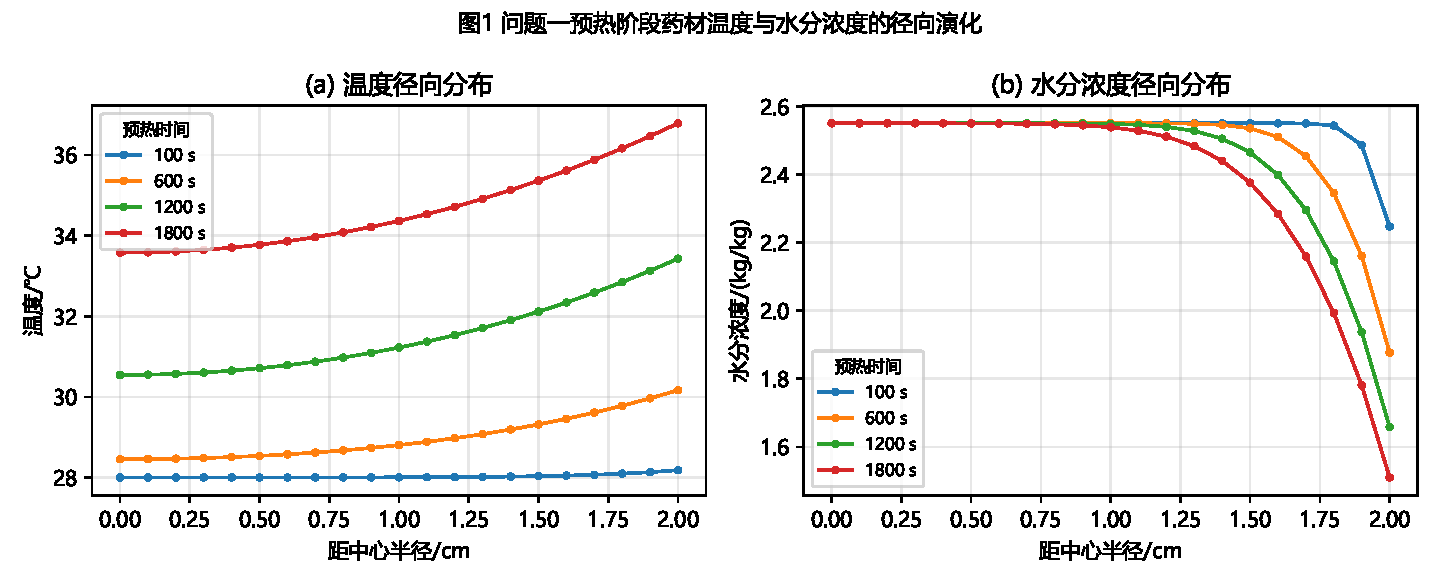
\includegraphics[width=0.88\textwidth]{../../results/paper_figures/fig1_problem1_radial.pdf}
  \caption{问题一预热阶段药材温度与水分浓度的径向演化。(a) $100\rm\,s$、$600\rm\,s$、$1200\rm\,s$ 与 $1800\rm\,s$ 的温度径向分布；(b) 对应时刻的水分浓度径向分布。温度自中心向表面升高并随时间整体上移；水分浓度在 $1800\rm\,s$ 内仅近表面区域明显下降，中心保持初值，表明传热明显快于水分扩散。}
  \label{fig:q1-radial}
\end{figure}

\begin{figure}[H]
  \centering
  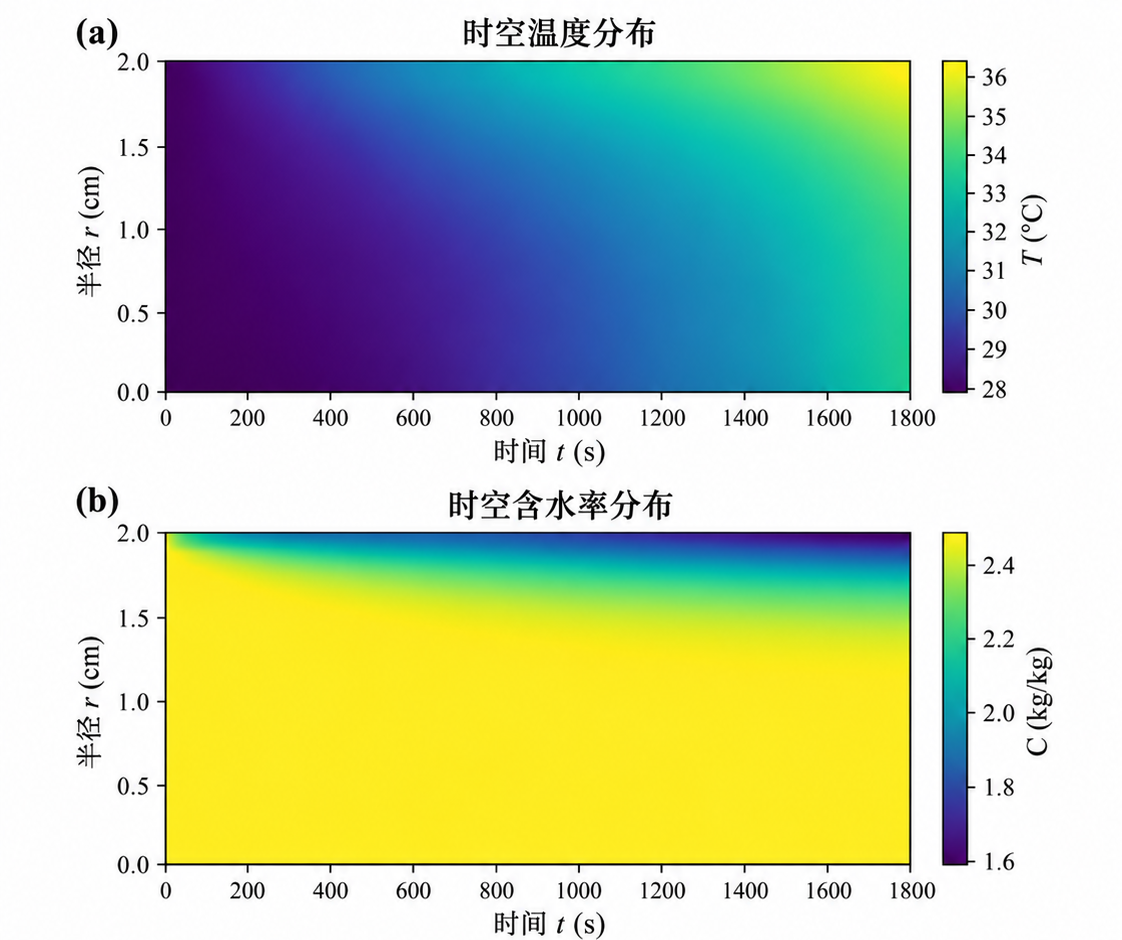
\includegraphics[width=0.75\textwidth]{../../results/paper_figures/insert_1_cn.png}
  \caption{预热平衡阶段（$0$--$1800\rm\,s$）药材内部温度场与含水率场沿径向位置的时空演化特征。子图 (a) 展示温度分布，子图 (b) 展示含水率分布。}
  \label{fig:temp_moisture_heatmap}
\end{figure}

图\ref{fig:temp_moisture_heatmap} 用二维时空热图展示了预热阶段药材内部热湿状态的演化。可以看出，表层区域首先升温，随后热量向中心传递，形成由表面到中心递减的温度梯度；含水率则先在外层下降，并逐渐向内部推进。上述现象与第三类边界条件下的物理过程一致：外部热风先作用于表面，内部传递速度受有限热扩散和水分扩散限制。该结果说明本文的一维轴对称模型能够刻画预热阶段的主要热湿迁移特征。

\subsection{本问小结与后续衔接}
问题一表明，即使在常物性预热阶段，药材内部也已形成不可忽略的径向梯度，后续模型不能采用整体均匀近似。由本问确定的几何处理、第三类边界和守恒型径向离散将直接用于问题二；区别在于问题二的物性随状态变化，温度场和水分场需要作为联合系统同步求解。

\section{问题二模型的建立与求解}
\subsection{本问任务与前文承接}
问题二仍在固定半径圆柱区域内计算，但物性关系由附录2常物性改为附录3经验式，并要求给出 $0.5$--$3.0\rm\,h$ 内若干位置的温度和水分浓度。与问题一相比，本问的关键变化是温度场和水分场不再相互独立：水分浓度会改变密度、比热容和热导率，温度又通过绝对温度项影响水分扩散系数。因此，本问沿用问题一建立的径向有限体积空间离散，但在时间推进时将温度和水分合并为联合状态，同步求解热湿耦合系统。

\subsection{模型建立}
附录3给出的状态相关物性如下：
\begin{equation}
  \rho(C)=650+128C,
\end{equation}
\begin{equation}
  c_p(C)=1450+\frac{2736C}{C+1},
\end{equation}
\begin{equation}
  k(C)=0.21+\frac{0.38C}{C+1},
\end{equation}
\begin{equation}
  D(C,T)=2.4\times10^{-3}\exp\left(-\frac{0.45}{C}\right)
  \exp\left(-\frac{3850}{T_K}\right),\qquad T_K=T+273.15.
\end{equation}
在该物性体系下，能量方程写为
\begin{equation}
  \rho(C)c_p(C)\frac{\partial T}{\partial t}
  =\frac1r\frac{\partial}{\partial r}
  \left[rk(C)\frac{\partial T}{\partial r}\right].
\end{equation}
水分迁移仍采用守恒型径向扩散方程：
\begin{equation}
  \frac{\partial C}{\partial t}
  =\frac1r\frac{\partial}{\partial r}
  \left[rD(C,T)\frac{\partial C}{\partial r}\right].
\end{equation}
初始条件和中心对称边界沿用问题一。表面边界中的物性取表面状态值，写为
\begin{equation}
  -k(C_s)\left.\frac{\partial T}{\partial r}\right|_{r=R}
  =h\left[T(R,t)-T_\infty(t)\right],
\end{equation}
\begin{equation}
  -D(C_s,T_s)\left.\frac{\partial C}{\partial r}\right|_{r=R}
  =h_m\left[C(R,t)-C_\infty(t)\right].
\end{equation}

\subsection{模型求解}
问题二仍采用严格径向守恒有限体积法进行空间离散。内部网格取 $\Delta r=0.025\rm\,cm$，共 81 个径向节点；温度和水分拼接后，联合状态维度为 162。控制体体积 $V_i=\pi(r_{i+1/2}^2-r_{i-1/2}^2)$、界面面积 $A_{i+1/2}=2\pi r_{i+1/2}$ 均按圆柱几何组装。界面热导率 $k$ 和扩散系数 $D$ 采用调和平均，以便在相邻控制体物性差异较大时保持通量计算稳定。

时间方向采用 \texttt{scipy.integrate.solve\_ivp} 中的自适应 BDF 隐式积分器。每次推进以上一时刻联合状态 $u^n=[T^n;C^n]$、附件1边界和附录3物性公式为基础，得到下一输出时刻联合状态 $u^{n+1}=[T^{n+1};C^{n+1}]$。计算设置为 $\mathrm{rtol}=2\times10^{-8}$，温度和水分的绝对容差分别为 $2\times10^{-9}$、$2\times10^{-10}$，最大内部步长为 $5\rm\,s$。由于 $T$ 与 $C$ 位于同一个状态向量内，BDF 在每个隐式步中同时处理热方程和水分方程的非线性残差，不再采用“先求温度、再求水分”的分步方式。为提高稳定性，非线性残差对应的块三对角稀疏 Jacobian 由解析式给出。

\begin{algorithm}[H]
  \SetAlgoLined
  构造径向 FVM 网格与控制体几何量 $V_i,A_{i\pm1/2}$\;
  由 $u^n$ 计算物性 $\rho(C),c_p(C),k(C),D(C,T+273.15)$\;
  界面 $k,D$ 取调和平均，组装严格守恒通量残差 $f(t,u)$\;
  中心控制体自然满足对称零通量，表面控制体加入 Robin 对流通量\;
  调用自适应 BDF 积分器（块三对角解析 Jacobian）推进至下一输出时刻\;
  \Return $u^{n+1}$\;
  \caption{问题二联合状态自适应 BDF 时间推进}
\end{algorithm}

BDF 积分覆盖 $0$--$3\rm\,h$，并输出 10801 个 $1\rm\,s$ 时刻。内部最大步长受 $5\rm\,s$ 上限约束，最小步长出现在初期薄边界层。为检验数值稳定性，本文将网格由 $\Delta r=0.025\rm\,cm$ 加密至 $0.0125\rm\,cm$，在 30 个论文采样点上得到温度最大绝对差 $4.16\times10^{-5}\rm\,{}^\circ\mathrm C$、水分最大绝对差 $4.67\times10^{-5}\rm\,kg/kg$。进一步收紧 BDF 容差并缩小最大步长后，温度最大绝对差为 $1.91\times10^{-5}\rm\,{}^\circ\mathrm C$，水分最大绝对差为 $4.84\times10^{-8}\rm\,kg/kg$。这些差异均低于四位小数显示精度，说明表\ref{tab:q2-temp} 和表\ref{tab:q2-moist} 的结果对网格和时间容差不敏感。

\subsection{结果分析}
表\ref{tab:q2-temp} 和表\ref{tab:q2-moist} 给出了问题二的计算结果。药材温度在前 $2\rm\,h$ 上升较快，随后逐渐接近烘房温度；到 $3\rm\,h$ 时，中心温度为 $49.8495^\circ\mathrm C$，表面温度为 $49.9664^\circ\mathrm C$，二者仅相差约 $0.1169^\circ\mathrm C$。相比之下，水分浓度的径向差异仍然明显：$3\rm\,h$ 时中心为 $1.7662\rm\,kg/kg$，表面为 $1.0081\rm\,kg/kg$，中心与表面相差 $0.7581\rm\,kg/kg$。因此，恒温干燥后期的主要限制不再是升温，而是内部水分向表面的扩散。

图\ref{fig:q2-heatmap} 从时空角度展示了上述差异。温度等值线主要集中在前半段，随后逐渐稀疏，说明温度场较快趋于准均匀；水分等值线则在整个 $3\rm\,h$ 内持续向中心推进，表明干燥前沿仍未到达中心区域。该结果也解释了问题三中停机时刻必须由全截面最大水分浓度控制，而不能用表面含水率代替。

\begin{table}[H]
  \centering
  \caption{3小时内药材的温度 $/^\circ\mathrm C$}
  \label{tab:q2-temp}
  \begin{tabular}{rrrrrr}
    \toprule
    时间/h & 0 cm & 0.5 cm & 1 cm & 1.5 cm & 2 cm\\ \midrule
    0.5 & 32.1893 & 32.3821 & 32.9659 & 33.9608 & 35.4131\\
    1.0 & 40.3816 & 40.5536 & 41.0605 & 41.8783 & 42.9977\\
    1.5 & 45.8468 & 45.9348 & 46.1930 & 46.6051 & 47.1401\\
    2.0 & 48.4502 & 48.4881 & 48.5985 & 48.7736 & 49.0034\\
    2.5 & 49.4670 & 49.4792 & 49.5137 & 49.5653 & 49.6609\\
    3.0 & 49.8495 & 49.8553 & 49.8746 & 49.9101 & 49.9664\\
    \bottomrule
  \end{tabular}
\end{table}

\begin{table}[H]
  \centering
  \caption{3小时内药材的水分浓度 $/\rm kg\cdot kg^{-1}$}
  \label{tab:q2-moist}
  \begin{tabular}{rrrrrr}
    \toprule
    时间/h & 0 cm & 0.5 cm & 1 cm & 1.5 cm & 2 cm\\ \midrule
    0.5 & 2.5499 & 2.5489 & 2.5255 & 2.3258 & 1.6486\\
    1.0 & 2.5257 & 2.4947 & 2.3578 & 2.0230 & 1.4711\\
    1.5 & 2.3860 & 2.3256 & 2.1344 & 1.8020 & 1.3475\\
    2.0 & 2.1708 & 2.1084 & 1.9236 & 1.6259 & 1.2311\\
    2.5 & 1.9566 & 1.9006 & 1.7360 & 1.4720 & 1.1166\\
    3.0 & 1.7662 & 1.7165 & 1.5702 & 1.3333 & 1.0081\\
    \bottomrule
  \end{tabular}
\end{table}

\begin{figure}[H]
  \centering
  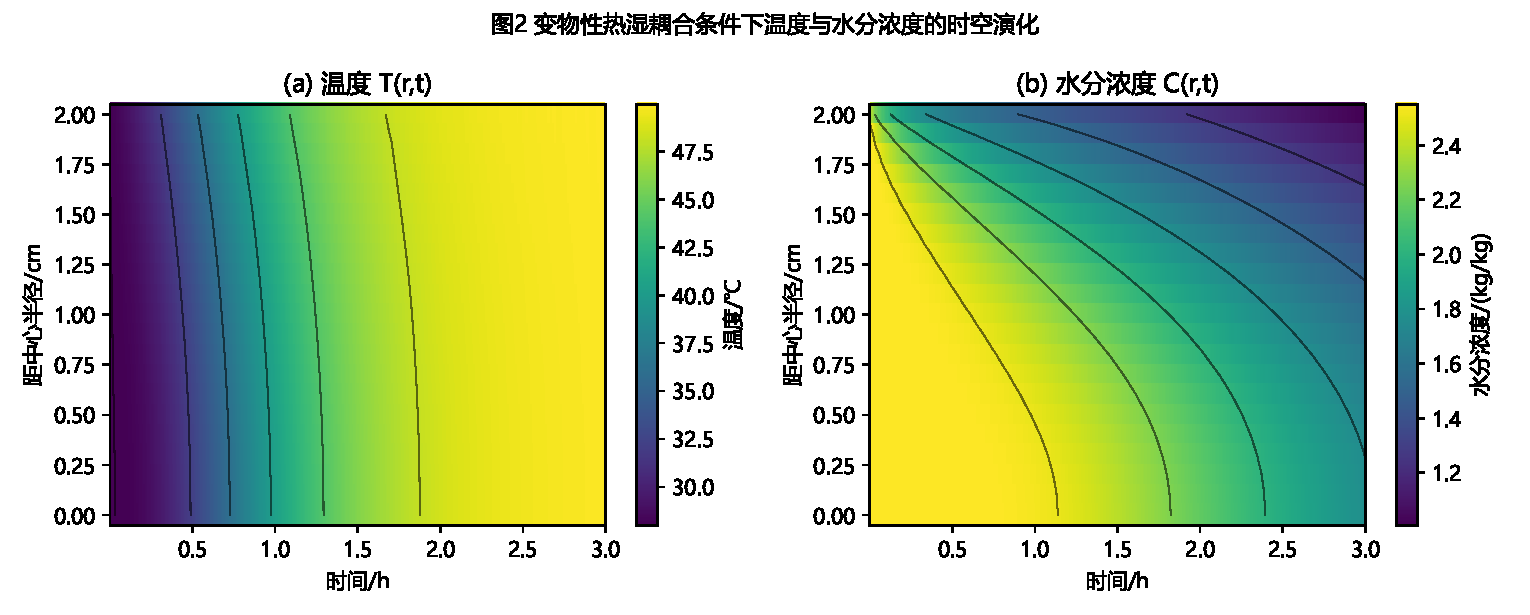
\includegraphics[width=0.88\textwidth]{../../results/paper_figures/fig2_problem2_heatmap.pdf}
  \caption{变物性热湿耦合条件下温度与水分浓度的时空演化。(a) 温度 $T(r,t)$；(b) 水分浓度 $C(r,t)$；黑色细线为等值线。温度场约 $2\rm\,h$ 内接近烘房温度、径向梯度消失；水分场在整个 $3\rm\,h$ 内保持明显径向梯度，说明恒温干燥阶段受内部水分扩散控制。}
  \label{fig:q2-heatmap}
\end{figure}

\subsection{本问小结与后续衔接}
问题二完成了由常物性预热模型向变物性热湿耦合模型的过渡。计算结果显示，三小时内温度趋于均匀的速度明显快于水分扩散，后续达标时间将主要受中心区域含水率控制。因此，问题三不需要重新建立控制方程，只需在本问耦合模型基础上继续积分，并加入全截面达标事件。

\section{问题三模型的建立与求解}
\subsection{本问任务与前文承接}
问题三沿用问题二的固定半径耦合模型，目标由给定时刻输出转为达标时间定位。题目要求药材“各处”水分浓度均低于 $0.15\rm\,kg/kg$，因此本文不使用表面值或平均值作停机标准，而采用全截面最大水分浓度判据。

\subsection{模型建立}
令固定半径区域为
\begin{equation}
  \Omega_R=\{r\mid 0\le r\le R,\ R=0.02\rm\,m\},
\end{equation}
并定义连续全域最大含水率
\begin{equation}
  C_{\max}(t)=\max_{r\in\Omega_R}C(r,t).
\end{equation}
达标时间写为
\begin{equation}
  t^*=\inf\{t\ge0: C_{\max}(t)<C_{\rm cr}\},\qquad C_{\rm cr}=0.15\rm\,kg/kg.
\end{equation}
数值离散后，径向节点集为 $\mathcal R_h=\{r_i\}_{i=0}^{N-1}$，相应离散判据为
\begin{equation}
  C_{\max,h}(t)=\max_{r_i\in\mathcal R_h}C_i(t),\qquad
  g_h(t)=C_{\max,h}(t)-C_{\rm cr}.
\end{equation}
当 $g_h(t)$ 由正变负时，药材全截面达到题设水分要求。由于径向扩散路径最长的位置在中心，计算中通常有
\begin{equation}
  C_{\max,h}(t)=C(0,t),
\end{equation}
该关系也可作为结果合理性的检查。热量方程、水分方程、初始条件和第三类边界均沿用问题二；外部边界在 $t>4\rm\,h$ 时取附件1末值恒定外推，即仍采用式(5.2)。

\subsection{模型求解}
本问仍采用径向守恒 FVM。生产网格取
\begin{equation}
  \Delta r=0.00078125\rm\,cm,
  \qquad N=2561,
\end{equation}
联合状态为
\begin{equation}
  u(t)=\bigl[T_0(t),\ldots,T_{N-1}(t),C_0(t),\ldots,C_{N-1}(t)\bigr]^{\mathsf T}.
\end{equation}
时间推进采用自适应 BDF，参数为
\begin{equation}
  \mathrm{rtol}=10^{-8},\qquad
  \mathrm{atol}_T=10^{-8},\qquad
  \mathrm{atol}_C=10^{-10},\qquad
  \Delta t_{\max}=30\rm\,s.
\end{equation}
连续事件函数取式(8.4)中的 $g_h(t)$，设置 \texttt{terminal=True}、\texttt{direction}$=-1$。积分器在步内定位
\begin{equation}
  g_h(t^*)=0,
\end{equation}
得到连续临界时间。题目要求的 Excel 输出采用 $60\rm\,s$ 时间网格，因此另定义离散输出达标时刻
\begin{equation}
  t_{60}=60\left\lceil\frac{t^*}{60}\right\rceil.
\end{equation}
二者分别对应“连续事件定位”和“结果文件首个达标行”，后文分开报告。

\begin{algorithm}[H]
  \SetAlgoLined
  构造严格径向 FVM 网格（$\Delta r=0.00078125\rm\,cm$，2561 节点）\;
  初始化联合状态 $u(0)=[T_0;C_0]$，$t=0$\;
  设置事件函数 $g_h(t)=\max_i C_i(t)-0.15$，方向 $-1$，\texttt{terminal=True}\;
  调用自适应 BDF 积分器（块三对角解析 Jacobian）推进\;
  在 $g_h(t)$ 变号处定位连续临界时间 $t^*$\;
  按 $60\rm\,s$ 输出网格保存水分场，并抽取到题目指定半径位置\;
  另用 backward-Euler + Picard 作双求解器交叉验证\;
  \caption{问题三达标停机求解流程}
\end{algorithm}

\subsection{结果分析}
在附件1末值外推边界下，连续事件定位给出
\begin{equation}
  t^*=205821.7420\rm\,s=57.1727\rm\,h.
\end{equation}
终止时刻最大水分浓度出现在中心点，且
\begin{equation}
  C_{\max,h}(t^*)=C(0,t^*)=0.1499888\rm\,kg/kg<C_{\rm cr}.
\end{equation}
由式(8.10)得到首个 $60\rm\,s$ 输出网格达标时刻
\begin{equation}
  t_{60}=205860\rm\,s=57.1833\rm\,h.
\end{equation}
因此，正文报告连续临界时间 $t^*$，结果文件末行采用 $t_{60}$。表\ref{tab:q3-moist} 中终止行中心值显示为 $0.1500$，来源于四舍五入；全精度值满足式(8.12)。

\begin{table}[H]
  \centering
  \caption{药材烘干过程的水分浓度 $/\rm kg\cdot kg^{-1}$}
  \label{tab:q3-moist}
  \begin{tabular}{rrrrrr}
    \toprule
    时间/h & 0 cm & 0.5 cm & 1 cm & 1.5 cm & 2 cm\\ \midrule
    6 & 1.0156 & 0.9868 & 0.9006 & 0.7546 & 0.5335\\
    12 & 0.4548 & 0.4418 & 0.4019 & 0.3289 & 0.1639\\
    18 & 0.2979 & 0.2906 & 0.2679 & 0.2247 & 0.0842\\
    24 & 0.2371 & 0.2321 & 0.2161 & 0.1851 & 0.0663\\
    30 & 0.2053 & 0.2013 & 0.1887 & 0.1637 & 0.0597\\
    36 & 0.1854 & 0.1821 & 0.1714 & 0.1501 & 0.0565\\
    42 & 0.1717 & 0.1687 & 0.1593 & 0.1404 & 0.0547\\
    48 & 0.1615 & 0.1588 & 0.1504 & 0.1332 & 0.0536\\
    54 & 0.1535 & 0.1511 & 0.1433 & 0.1275 & 0.0528\\
    57.1727 & 0.1500 & 0.1477 & 0.1402 & 0.1249 & 0.0525\\
    \bottomrule
  \end{tabular}
\end{table}

表\ref{tab:q3-moist} 中，表面点在 $18\rm\,h$ 已降至 $0.0842\rm\,kg/kg$，中心点仍为 $0.2979\rm\,kg/kg$；到 $54\rm\,h$，表面点为 $0.0528\rm\,kg/kg$，中心点仍为 $0.1535\rm\,kg/kg$。这说明固定半径模型的停机时间主要由中心控制，可概括为
\begin{equation}
  C(R,t)<C_{\rm cr}\ \not\Rightarrow\ C_{\max}(t)<C_{\rm cr}.
\end{equation}
图\ref{fig:q3-event} 中，$C=C_{\rm cr}$ 等值线由表面向中心收缩，进一步说明干燥前沿自外向内推进；连续临界时间 $t^*$ 和离散输出时刻 $t_{60}$ 分别对应式(8.11)和式(8.13)。

\begin{figure}[H]
  \centering
  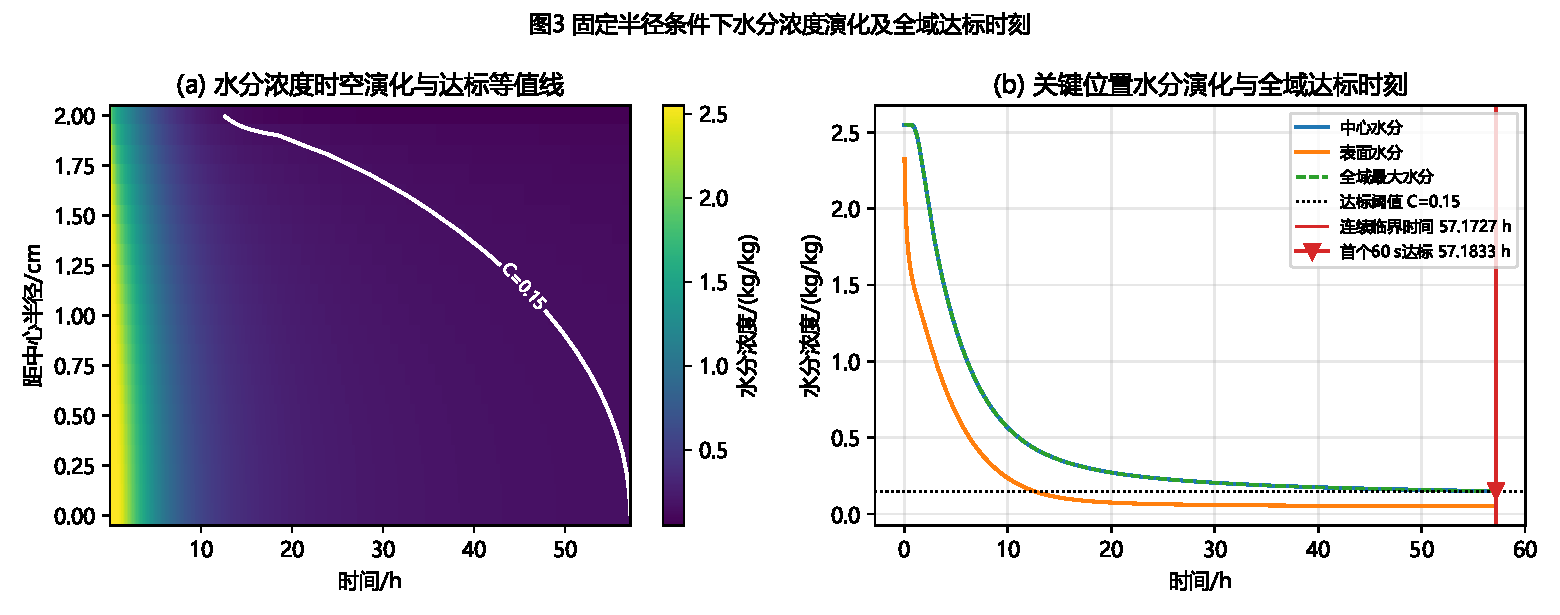
\includegraphics[width=0.88\textwidth]{../../results/paper_figures/fig3_problem3_event.pdf}
  \caption{固定半径条件下水分浓度演化及全域达标时刻。(a) 水分浓度时空热力图，白色曲线为 $C=0.15\rm\,kg/kg$ 达标等值线；(b) 中心、表面与全域最大水分随时间演化，水平点线为达标阈值，竖线与三角标记分别给出连续临界时间与首个 $60\rm\,s$ 达标时刻。}
  \label{fig:q3-event}
\end{figure}

为区分边界假设与数值误差，记边界情景集合为
\begin{equation}
  \mathcal S=\{(\Delta T_\infty,\eta_C):\Delta T_\infty\in\{-2,0,2\},\ \eta_C\in\{0.9,1.0,1.1\}\}.
\end{equation}
在该集合上重算得
\begin{equation}
  t^*(\mathcal S)\in[53.6154,61.0702]\rm\,h.
\end{equation}
若只扰动 $h_m$ 的 $\pm10\%$，则
\begin{equation}
  t^*\in[56.5955,57.9086]\rm\,h.
\end{equation}
而数值误差量级为
\begin{equation}
  |t^*_{\rm BDF}-t^*_{\rm BE}|=7.95\rm\,s,
  \quad |t^*_h-t^*_{\rm Rich}|\approx10\rm\,s,
  \quad |t^*_{h}-t^*_{2h}|=39.34\rm\,s.
\end{equation}
可见，边界外推带来的小时级变化显著大于数值离散误差。因此，$57.1727\rm\,h$ 是末值外推边界下的点估计，式(8.16)用于描述外部边界不确定性。

\subsection{本问小结与后续衔接}
问题三在固定半径、附录3物性和末值外推边界下得到
\begin{equation}
  t^*=57.1727\rm\,h,\qquad t^*(\mathcal S)\in[53.6154,61.0702]\rm\,h.
\end{equation}
该结果构成问题四移动边界模型的固定半径基准。问题四将在同一全截面判据下引入 $R(t)$ 和附录4物性，比较收缩对达标时间的影响。
\section{问题四模型的建立与求解}
\subsection{本问任务与前文承接}
问题四在问题三达标停机框架上进一步引入半径收缩。与问题三相比，本问同时发生两类变化：物性关系由附录3改为附录4，几何边界由固定半径 $R=2.0\rm\,cm$ 改为附件2给定的时变半径 $R(t)$。半径收缩会改变扩散距离和表面位置，若仍在物理半径上直接离散，需要不断移动网格。为保持计算网格稳定，本文将移动物理域映射到固定计算域，并在相同全截面含水率阈值下求解临界时间。

\subsection{建模思路}
移动边界处理的核心，是把随时间变化的物理区间 $r\in[0,R(t)]$ 化为固定区间。本文采用 Landau 前置固定变换，引入物质坐标
\begin{equation}
  \xi=\frac{r}{R(t)}\in[0,1],
\end{equation}
从而把收缩域映射到 $\xi\in[0,1]$。在均匀径向收缩假设下，$\xi$ 表示同一物质层的位置标签；干基含水率 $C$ 以单位干物质质量为基准，也适合在物质坐标下跟踪。对守恒式作物质导数处理后，收缩效应主要体现在两个位置：内部扩散项出现尺度因子 $1/R^2(t)$，表面通量项出现尺度因子 $R(t)$。在该物质坐标解释下，方程中不另加网格对流项。

需要说明的是，附件2的 $R(t)$ 在本文中作为题目给定的经验输入，并非由含水率场反推的未知量。附录4密度律与附件2半径轨迹是否同时满足干物质闭合，不作为本问求解的约束条件；该一致性问题在后文模型检验与评价中单独讨论。

\subsection{模型建立}
附录4给出的状态相关物性为
\begin{equation}
  \rho(C)=760+90C,\qquad
  c_p(C)=1850+\frac{2150C}{C+1},\qquad
  k(C)=0.12+\frac{0.20C}{C+1},
\end{equation}
\begin{equation}
  D(C,T)=4.2\times10^{-4}\exp\left(-\frac{0.30}{C}\right)
  \exp\left(-\frac{3850}{T_K}\right),\qquad T_K=T+273.15.
\end{equation}
在物质坐标 $\xi$ 下，温度场与水分场可统一写为压缩扩散方程：
\begin{equation}
  \left.\frac{\partial u}{\partial t}\right|_{\xi}
  =\frac{1}{\mathrm{cap}\cdot\xi R^2}
  \frac{\partial}{\partial\xi}\left(\xi\,\mathrm{cond}\,\frac{\partial u}{\partial\xi}\right),
\end{equation}
其中 $u=T$ 时 $\mathrm{cap}=\rho(C)c_p(C)$、$\mathrm{cond}=k(C)$；$u=C$ 时 $\mathrm{cap}=1$、$\mathrm{cond}=D(C,T)$；$R(t)$ 由附件2线性插值得到。初始条件为 $T(\xi,0)=28$、$C(\xi,0)=2.55$。中心 $\xi=0$ 为对称零通量边界；表面 $\xi=1$（即 $r=R(t)$）为第三类边界
\begin{equation}
  -\mathrm{cond}\left.\frac{\partial u}{\partial\xi}\right|_{\xi=1}
  =\mathrm{transfer}\cdot R(t)\cdot\left(u_s-u_{\rm ext}\right),
\end{equation}
其中温度场 $\mathrm{transfer}=h$、$u_{\rm ext}=T_\infty(t)$，水分场 $\mathrm{transfer}=h_m$、$u_{\rm ext}=C_\infty(t)$。$4\rm\,h$ 后的烘房边界与问题三一致，取附件1末值恒定外推。

收缩和物性切换对达标时间的影响方向并不完全相同。半径收缩通过 $1/R^2(t)$ 增大有效扩散尺度，并缩短中心到表面的距离；而附录4中的扩散系数基值 $4.2\times10^{-4}$ 小于附录3中的 $2.4\times10^{-3}$，会降低相同状态下的水分迁移速率。二者共同决定本问相对于问题三是提前还是延后达标。停机判据仍取全剖面最大水分浓度，首次满足 $C_{\max}(t)<0.15\rm\,kg/kg$ 时停止积分。

\subsection{模型求解}
问题四在固定 $\xi$ 网格上采用严格径向守恒有限体积法。计算条件包括初值 $T_0,C_0$、附录4物性、附件1环境边界及末值外推规则，以及附件2半径序列 $R(t)$；计算结果包括连续临界时间 $t^*$ 和含移动表面列的水分浓度过程表。生产配置取 $N=3201$ 个 $\xi$ 节点，$\Delta\xi=1/(N-1)$；控制体几何量取 $\hat V_i=\frac12(\xi_{i+1/2}^2-\xi_{i-1/2}^2)$，界面面积取 $\hat A_{i+1/2}=\xi_{i+1/2}$，相当于在单位 $\xi$ 圆盘上组装径向守恒通量。界面热导率 $k$ 和扩散系数 $D$ 均采用调和平均，以降低强梯度区域的界面通量高估风险。

时间推进仍采用 \texttt{scipy.integrate.solve\_ivp} 的联合状态自适应 BDF 隐式积分器。计算参数为 $\mathrm{rtol}=10^{-8}$，温度和水分绝对容差分别为 $10^{-8}$ 与 $10^{-10}$，最大内部步长为 $30\rm\,s$。每个时间步由附件2线性插值得到当前 $R(t)$，并据此更新有效扩散系数 $\mathrm{cond}/R^2$ 和表面对流尺度 $\mathrm{transfer}\cdot R$。中心 $\xi=0$ 用对称零通量条件消除奇点，表面 $\xi=1$ 施加第三类边界；块三对角稀疏 Jacobian 由解析式提供。终止事件设为 $g(t)=\max_\xi C(\xi,t)-0.15$，其中 \texttt{terminal=True}，\texttt{direction}$=-1$。为验证物质坐标实现，程序还进行了 $D=0$ 时物质剖面守恒自检，并以 backward-Euler + Picard 固定步隐式格式作为独立对照。

\begin{algorithm}[H]
  \SetAlgoLined
  构造固定 $\xi$ 网格（$N=3201$），初始化联合状态 $u(0)=[T_0;C_0]$，$t=0$\;
  定义终止事件 $g(t)=\max_\xi C(\xi,t)-0.15$，方向 $-1$，\texttt{terminal=True}\;
  \While{积分器未触发终止事件}{
    由附件2插值取当前 $R(t)$\;
    由 $u$ 计算物性 $\rho(C),c_p(C),k(C),D(C,T+273.15)$\;
    界面 $k,D$ 取调和平均，组装 $\xi$ 系压缩扩散通量残差（扩散乘 $1/R^2$、表面对流乘 $R$）\;
    调用自适应 BDF 积分器（块三对角解析 Jacobian）推进\;
    若到达 $60\rm\,s$ 输出间隔，按固定距离 $d=\xi R(t)$ 记录水分浓度，$d>R(t)$ 处置空\;
  }
  输出 $t^*$ 及终止时刻水分浓度\;
  另用 backward-Euler + Picard 作双求解器交叉验证\;
  \caption{问题四移动边界达标停机求解流程}
\end{algorithm}

BDF 积分触发终止事件后得到连续临界时间。内部通量平衡的最大归一化残差为 $2.087\times10^{-16}$，处于机器精度量级；最小原始水分为 $0.0525\rm\,kg/kg$，计算过程中未触发非负裁剪；全域最大含水率始终位于中心 $\xi=0$，与圆柱径向扩散的滞后规律一致。backward-Euler + Picard 对照在 $\Delta t=20/10/5/2.5\rm\,s$ 四档时间步下分别给出 $t^*=50.8377/50.8312/50.8279/50.8262\rm\,h$，随时间步减小向 BDF 结果收敛；最细 BE 与 BDF 相差 $6.15\rm\,s$，相对差为 $3.36\times10^{-5}$。

\subsection{结果分析}
计算得到
\begin{equation}
  t^*=182968.2250\rm\,s=50.8245\rm\,h.
\end{equation}
半径从首次采样时刻的 $1.9958\rm\,cm$ 收缩到临界时刻的约 $1.2000\rm\,cm$。临界时刻中心全精度含水率已低于 $0.15\rm\,kg/kg$，表中显示 $0.1500$ 来自四舍五入。第一个在 $60\rm\,s$ 输出网格上严格达标的时刻为 $183000\rm\,s=50.8333\rm\,h$，即 \texttt{result4.xlsx} 的末行。表\ref{tab:q4-moist} 按题目要求给出每 $6\rm\,h$ 及临界时刻、固定距离 $0$、$0.5$、$1\rm\,cm$ 与移动表面处的水分浓度。由于半径在后期已降至 $1.5\rm\,cm$ 以下，更远的固定距离已不在药材内部，该处状态应由烘房环境而非药材内部方程描述，故表中不再列出，不属于数据缺失。

\begin{table}[H]
  \centering
  \caption{药材烘干过程的水分浓度（含半径收缩·移动表面）$/\rm kg\cdot kg^{-1}$}
  \label{tab:q4-moist}
  \begin{tabular}{rrrrr}
    \toprule
    时间/h & 0 cm & 0.5 cm & 1 cm & 药材表面\\ \midrule
    6 & 1.7172 & 1.5357 & 1.0217 & 0.4217\\
    12 & 0.7343 & 0.6518 & 0.4069 & 0.1667\\
    18 & 0.4066 & 0.3668 & 0.2388 & 0.0889\\
    24 & 0.2837 & 0.2599 & 0.1783 & 0.0671\\
    30 & 0.2253 & 0.2085 & 0.1488 & 0.0593\\
    36 & 0.1921 & 0.1790 & 0.1312 & 0.0558\\
    42 & 0.1706 & 0.1598 & 0.1196 & 0.0539\\
    48 & 0.1556 & 0.1463 & 0.1113 & 0.0529\\
    50.8245 & 0.1500 & 0.1413 & 0.1081 & 0.0525\\
    \bottomrule
  \end{tabular}
\end{table}

\begin{figure}[H]
  \centering
  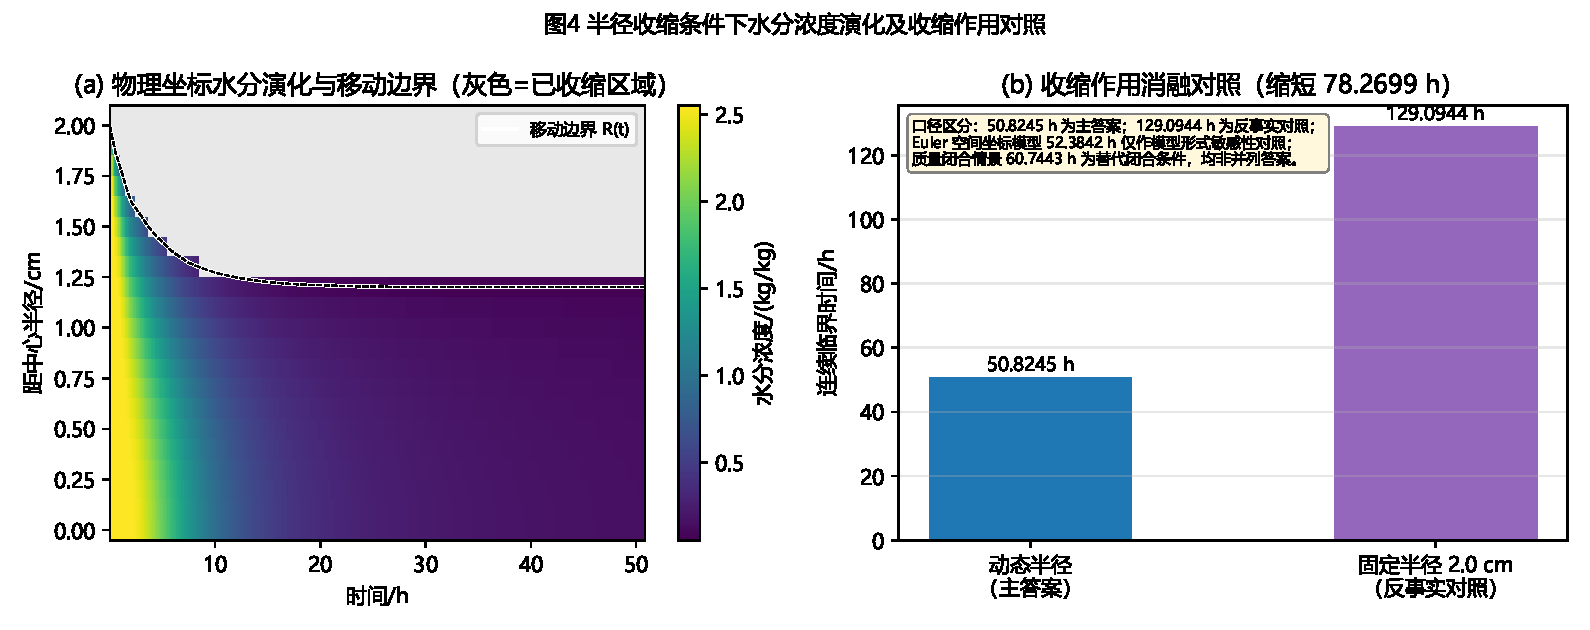
\includegraphics[width=0.88\textwidth]{../../results/paper_figures/fig4_problem4_moving_boundary.pdf}
  \caption{半径收缩条件下水分浓度演化及收缩作用对照。(a) 物理坐标下水分浓度热力图，白色曲线为移动边界 $R(t)$，灰色为已收缩退出的药材区域；(b) 相同附录4物性与边界条件下动态半径与固定半径 $2.0\rm\,cm$ 的连续临界时间消融对照，图内方框给出各对照值与主答案的口径区分。}
  \label{fig:q4-moving}
\end{figure}

问题三在固定半径下的终止时间为 $57.1727\rm\,h$；问题四引入半径收缩和附录4物性后，终止时间为 $50.8245\rm\,h$。两问同时改变了物性公式和几何边界，因此二者之差不能直接解释为单纯的收缩贡献。为分离收缩效应，本文在附录4物性和边界条件均不变的前提下作消融对照：若仍固定半径为 $2.0\rm\,cm$，连续临界时间为 $129.0944\rm\,h$，比动态半径结果延长 $78.2699\rm\,h$（图\ref{fig:q4-moving}(b)）。这说明在附录4物性条件下，半径收缩显著缩短了扩散路径，是本问达标时间提前的主要原因。

图\ref{fig:q4-moving}(a) 中，移动边界 $R(t)$ 从 $2.0\rm\,cm$ 收缩至临界时刻的约 $1.2\rm\,cm$，灰色区域为已收缩退出的药材区域。剩余区域内水分浓度仍呈中心高、表面低的分布形态；表面含水率后期接近 $0.0525\rm\,kg/kg$，与环境末值 $0.04986\rm\,kg/kg$ 相近，而中心含水率下降较慢并继续控制终止时刻。需要强调的是，$129.0944\rm\,h$ 仅为固定半径下的反事实对照，Euler 空间坐标模型 $52.3842\rm\,h$ 与质量闭合情景 $60.7443\rm\,h$ 分别属于模型形式敏感性与替代闭合条件结果，均不与 $50.8245\rm\,h$ 构成并列答案。

边界情景分析给出了默认答案的外部适用范围。将 $4\rm\,h$ 后温度扰动 $\pm2^\circ\mathrm C$、水分扰动 $\pm10\%$ 组成 $3\times3$ 情景时，$t^*$ 落在 $47.6834$--$54.2753\rm\,h$；传质系数 $h_m$ 扰动 $\pm10\%$ 时，$t^*$ 落在 $50.6035$--$51.1159\rm\,h$；用附件最后 $30$ 分钟或 $1\rm\,h$ 均值延拓代替末值外推时，$t^*$ 为 $51.0757$--$51.0972\rm\,h$。与这些小时量级的边界差异相比，数值离散误差较小：网格 $201\to3201$ 的末级差为 $3.30\rm\,s$，BDF 容差三档差小于 $2\times10^{-4}\rm\,s$，BDF 与 BE-Picard 对照差为 $6.15\rm\,s$。因此，$50.8245\rm\,h$ 可作为题设默认边界下的点估计，边界情景区间用于说明后期烘房条件外推带来的不确定性。

\subsection{本问小结与后续衔接}
问题四通过物质坐标前置固定，将半径收缩问题转化为固定域上的压缩扩散问题，并在同一全截面达标判据下得到连续临界时间 $t^*=50.8245\rm\,h$。该时间短于问题三固定半径结果 $57.1727\rm\,h$，说明在题设半径轨迹和附录4物性下，扩散路径缩短带来的加速作用占主导。后续模型检验与评价将进一步讨论数值收敛、坐标解释差异以及附件2半径轨迹与附录4密度律之间的闭合关系。

\section{模型检验与稳定性分析}
\subsection{数值收敛检验}
为判断计算结果是否主要由模型输入决定，而非由离散误差造成，本文从空间网格、时间积分和独立求解器三个方面进行检验。问题一采用 $\Delta r=0.0025\rm\,cm$ 的内部网格，共 801 个径向节点，已经细于题目要求的输出网格。将网格继续加密至 $\Delta r=0.00125\rm\,cm$ 后，在全部 $1801\times21$ 个输出格上，温度最大变化为 $1.71\times10^{-4}{}^\circ\mathrm C$，水分最大变化为 $1.90\times10^{-4}\rm\,kg/kg$。最大水分差出现在 $t=1\rm\,s$ 的表面位置，对应初始高含水率药材与低湿环境接触时形成的极薄边界层；正文表格从 $100\rm\,s$ 起采样，因此该局部差异不影响四位小数结果。界面扩散系数由算术平均改为调和平均后，温度场不变，水分场最大变化为 $2.56\times10^{-7}\rm\,kg/kg$，低于报告精度。

问题二和问题三均采用联合状态 BDF 推进，并保留后向欧拉--Picard 格式作为求解器对照。对问题二，在表\ref{tab:q2-temp}、表\ref{tab:q2-moist} 的 30 个采样点上检验，内部网格由 $0.025\rm\,cm$ 加密至 $0.0125\rm\,cm$ 后，温度最大差为 $4.16\times10^{-5}{}^\circ\mathrm C$，水分最大差为 $4.67\times10^{-5}\rm\,kg/kg$；将 BDF 相对容差由 $2\times10^{-8}$ 收紧至 $10^{-9}$，并把最大内部步长由 $5\rm\,s$ 缩小至 $2\rm\,s$ 后，论文表格采样值在四位小数下保持不变。对问题三，达标时间对空间离散更敏感，本文从 $\Delta r=0.1\rm\,cm$ 逐级加密至 $0.00078125\rm\,cm$。末两级连续事件时间差为 $39.34\rm\,s$，相对差 $1.911\times10^{-4}$；由末三层估计的观察收敛阶为 $p=2.30$，Richardson 外推值为 $205811.7290\rm\,s$，生产网格结果比外推值高 $10.01\rm\,s$。BDF 容差取 $10^{-7}$、$10^{-8}$、$10^{-9}$ 时，事件时间差为 $1.5\times10^{-4}\rm\,s$；最严格 BDF 与 $\Delta t=2.5\rm\,s$ 后向欧拉结果相差 $7.95\rm\,s$。问题三水分守恒残差为 $1.08\times10^{-16}$，未触发非负裁剪，径向剖面保持单调。

需要强调的是，调和平均必须与足够细的网格共同使用。在 $\Delta r=0.1\rm\,cm$ 的粗网格上直接使用调和平均，会得到 $557.4748\rm\,h$ 的异常终止时间。这一现象并非物理停机时间，而是粗网格将表层低扩散区压缩到单个界面阻力上，放大了干燥前沿阻力。随网格逐级加密（$\Delta r=0.05$、$0.025$、$0.0125$、$0.00625$、$0.003125$、$0.0015625$、$0.00078125\rm\,cm$），终止时间依次回落到 $226.5453$、$88.1319$、$60.2157$、$57.5648$、$57.2375$、$57.1836$、$57.1727\rm\,h$。因此，调和平均在本文中是细网格守恒离散的一部分，而不是单独的经验修正。

问题四在物质坐标 $\xi$ 网格上进行同样的收敛检验。节点数 $N$ 从 201 加密至 3201 时，连续临界时间依次为 $50.9091$、$50.8442$、$50.8291$、$50.8254$、$50.8245\rm\,h$，相邻差为 $-233.59$、$-54.43$、$-13.27$、$-3.30\rm\,s$，故生产配置取 $N=3201$。BDF 相对容差取 $10^{-7}$、$10^{-8}$、$10^{-9}$ 时，结果为 $50.824506$、$50.824507$、$50.824507\rm\,h$，最大差小于 $2\times10^{-4}\rm\,s$。后向欧拉--Picard 在 $\Delta t=20$、$10$、$5$、$2.5\rm\,s$ 下分别给出 $50.8377$、$50.8312$、$50.8279$、$50.8262\rm\,h$，随步长缩小向 BDF 结果收敛；最细后向欧拉与 BDF 相差 $6.15\rm\,s$。问题四离散通量平衡残差为 $2.087\times10^{-16}$，全域最大含水率始终位于中心 $\xi=0$。上述数值差异均处于秒级，明显低于后文边界情景给出的小时级变化。

\subsection{问题四两种坐标模型的结果比较}
问题四主模型采用物质坐标 FVM-BDF 格式。由于题目只给出整体半径变化，没有给出内部形变速度场，移动边界方程的坐标解释会带来额外模型不确定性。为评估这一因素，本文另计算 Euler 空间坐标模型作为敏感性对照。表\ref{tab:q4-coord}用于比较两种模型口径，不表示在两个结果之间按数值大小择优。

\begin{table}[htbp]
  \centering
  \caption{问题四两种坐标模型的结果比较}
  \label{tab:q4-coord}
  \small
  \begin{tabular}{lcp{6.5cm}}
    \toprule
    模型 & $t^*$/h & 说明\\
    \midrule
    物质坐标 FVM-BDF 模型 & \textbf{50.8245} & 问题四最终结果\\
    Euler 空间坐标模型 & 52.3842 & 坐标处理敏感性对照，不纳入主答案\\
    \bottomrule
  \end{tabular}
\end{table}

物质坐标模型以 $\xi=r/R(t)$ 标记同一物质层，变换后不含网格对流项，符合本文对均匀径向收缩的主假设。Euler 空间坐标模型保留收缩对流项 $(\xi R'/R)\,\partial u/\partial\xi$，得到临界时间 $52.3842\rm\,h$，比主模型晚 $1.5597\rm\,h$。这一差异反映的是内部形变场未知带来的模型形式敏感性。相比之下，固定步后向欧拉--Picard 与 FVM-BDF 主模型相差 $0.0301\rm\,h$，约为 $0.06\%$；该实现差异小于坐标解释差异，也小于后期边界外推造成的情景范围。

\subsection{边界敏感性讨论}
问题三和问题四的计算时间分别为 $57.1727\rm\,h$ 与 $50.8245\rm\,h$，均远超过附件1覆盖的前 $4\rm\,h$。因此，默认计算中的多数积分时间依赖 $4\rm\,h$ 后边界末值外推，而不再由实测边界直接约束。边界敏感性分析的目的，是把这一外部假设与前述数值离散误差分开。

本文对问题三和问题四各设置三组情景，均使用生产网格与 BDF 配置，只改变 $4\rm\,h$ 后边界或传质系数。第一组将后期温度扰动 $\pm2^\circ\mathrm C$、后期环境水分扰动 $\pm10\%$ 作 $3\times3$ 组合：问题三 $t^*\in[53.6154,61.0702]\rm\,h$，问题四 $t^*\in[47.6834,54.2753]\rm\,h$。在固定温度下，环境水分 $\pm10\%$ 只造成约 $6$--$11$ 分钟变化，说明后期温度是主要边界驱动。第二组扰动传质系数 $h_m$ 的 $\pm10\%$，问题三给出 $[56.5955,57.9086]\rm\,h$，问题四给出 $[50.6035,51.1159]\rm\,h$。第三组用附件最后 $30$ 分钟或最后 $1\rm\,h$ 的时间平均值代替末点值，问题三得到 $[57.1727,57.4829]\rm\,h$，问题四得到 $[51.0757,51.0972]\rm\,h$。

这些情景区间处于小时量级，而网格、BDF 容差和双求解器带来的差异主要为秒级。因而，问题三的 $57.1727\rm\,h$ 和问题四的 $50.8245\rm\,h$ 应理解为末值外推边界下的点估计；边界情景范围用于描述外部边界假设的敏感性，不具有统计置信区间含义。问题四表格只列至 $1\rm\,cm$ 固定距离加移动表面，是因为半径在后期降至 $1.5\rm\,cm$ 以下，更远的固定距离已不在药材内部，故不属于数据缺失。

\subsection{物理合理性检验}
四个问题的结果在物理顺序上保持一致：表面率先受外部热风影响，中心区域响应滞后。问题一中表面升温和脱水均快于中心；问题二中温度场趋于均匀后，水分场仍保留径向梯度；问题三中表面较早接近低含水率，中心点控制最终停机时刻；问题四中半径收缩缩短传质路径，使终止时间短于固定半径基准。该序列与圆柱径向扩散和收缩移动边界的基本图像相符，也与全截面最大含水率作为停机判据的设置一致。

\section{模型评价}
\subsection{模型优点}
本文模型的主要优点在于框架统一、判据严格、检验充分。首先，四个问题均在径向守恒有限体积框架下展开，从常物性预热、变物性耦合到固定半径达标和收缩移动边界，几何口径保持一致。各问只替换物性、边界时长、终止事件或半径函数，减少了重复建模造成的参数口径漂移。

其次，问题二至问题四把温度场和水分场作为联合状态整体推进，能够在隐式步内同步处理状态相关物性。界面热导率和扩散系数采用调和平均，并配合细网格处理后期低扩散边界层中的通量变化。停机判据采用全截面最大水分浓度，并通过连续事件 $g(t)=\max(C)-0.15$ 定位临界时刻，比表面含水率、平均含水率或固定 $60\rm\,s$ 输出网格更严格，能够避免中心区域尚未达标时提前停机。

最后，本文对数值误差和模型假设分别进行检验。问题三和问题四的最大归一化水分守恒残差分别为 $1.08\times10^{-16}$ 和 $2.087\times10^{-16}$，径向剖面保持单调。问题三生产网格与 Richardson 外推差 $10.01\rm\,s$，问题四末级网格差 $3.30\rm\,s$，BDF 与后向欧拉对照差 $6.15\rm\,s$。这些秒级差异低于边界情景造成的小时级变化，说明主要结论不依赖某一特定离散设置。对于 $4\rm\,h$ 后边界外推和问题四坐标解释，本文也给出敏感性对照，使默认点估计和适用范围能够同时呈现。

\subsection{模型不足}
本文模型仍有三类主要不足。第一，模型没有显式加入蒸发潜热源项。题目只给出 Fourier 导热、Fick 扩散方程组以及 $h,h_m,D$ 等参数，未给出汽化潜热 $L_v$、蒸发速率律和气相输运闭合关系，因此难以在题设数据内构造可核验的潜热耦合项。若按外部文献值 $L_v\approx2260\rm\,kJ/kg$ 作量级估算，全程失水约 $0.852\rm\,kg/m$，潜热需求约 $1.93\rm\,MJ/m$，而给定换热条件下对流显热约 $4.70\times10^{4}\rm\,J/m$，二者相差约 $41$ 倍。用等效蒸发冷却代理潜热效应时，温度降低会使 $D\propto\exp(-3850/T_K)$ 减小，干燥过程变慢，干物质诊断指标的相对变幅由 $28.02\%$ 增至约 $30.16\%$（等效温降 $5\rm\,K$）。这些计算只用于说明潜热闭合缺失的量级和方向，不用于修正 $50.8245\rm\,h$ 主答案。

第二，问题三和问题四在 $4\rm\,h$ 后采用附件1末值恒定外推。该假设对应的问题三情景范围为 $53.6154$--$61.0702\rm\,h$，问题四为 $47.6834$--$54.2753\rm\,h$，构成外部边界层面的主要不确定源。该不确定性来自题设边界数据时长不足，继续压低网格误差无法消除。另一个局部数值边界是问题二最初几秒的表面薄边界层：主计算网格为 $0.025\rm\,cm$，在 $t=1\rm\,s$ 表面水分与加密网格相差约 $0.005\rm\,kg/kg$。正文表格从 $0.5\rm\,h$ 起采样，不受该局部误差影响；若后续需要使用秒级近表面含水率，则应采用局部加密或自适应网格重算。

第三，问题四存在收缩轨迹与密度经验式之间的口径张力。干物质质量诊断指标在全程的相对变化范围为 $28.02\%$，而求解器误差和离散误差不足以解释该变幅。进一步分解可知，指标 $\kappa$ 等于几何因子 $G=(R/R_0)^2$ 与组成因子 $S$ 的乘积；其最小值 $\kappa_{\min}=0.7198$ 出现在约 $7\rm\,h$。终止时由附录4密度律和模拟水分场得到的平均干基密度为 $689.30\rm\,kg/m^3$，而干物质闭合在 $R(t^*)\approx1.2\rm\,cm$ 下要求 $774.26\rm\,kg/m^3$，缺口约 $11.0\%$。附录4的整体密度 $\rho(C)=760+90C$ 与干基含水率定义共同蕴含 $\rho_s(C)=\rho/(1+C)=90+670/(1+C)$，在 $C\ge0$ 下上确界仅为 $760\rm\,kg/m^3$；而干物质闭合要求 $\rho_s=\rho_{s0}(R_0/R)^2$，对应临界半径 $R_c=1.2112\rm\,cm$。附件2半径自约 $19.5\rm\,h$ 起低于该临界值，若仍要求闭合，则需负含水率。由此可见，该闭合矛盾属于题设经验半径轨迹与附录4密度律之间的模型形式差异，不能通过加密网格消除。若反向构造满足干物质闭合的自洽收缩轨迹，诊断计算给出 $t^*\approx60.7443\rm\,h$，比主模型 $50.8245\rm\,h$ 延后约 $9.92\rm\,h$。因此，本文保留题目给定 $R(t)$ 下的 $50.8245\rm\,h$ 作为主答案，将 $60.74\rm\,h$ 作为收缩--密度闭合口径下的模型形式上界。

\subsection{模型改进方向}
后续改进应优先补足对结论影响最大的物理和边界信息。若能够获得 $4\rm\,h$ 后恒温干燥段的实际温湿设定，应先替换末值外推边界并重算问题三、问题四；这一步直接对应当前小时级边界敏感性区间。若题目补充汽化潜热、蒸发速率律或气相输运参数，可在温度方程中加入可识别的相变源项，避免用等效冷却近似潜热影响。对问题四而言，更关键的是同步获得半径、质量和含水率实验数据，用以判断附件2半径轨迹与附录4密度律之间的闭合缺口来自经验式误差、收缩测量口径差异，还是需要引入独立的结构变量。数值方法方面，可进一步加入制造解法、半解析算例或更高阶刚性积分器交叉验证；但在现有题设条件下，继续压低秒级离散误差对主结论的收益低于改进外部边界和物理闭合信息。

\section{结论}
本文针对圆柱药材热风烘干过程，建立了由常物性预热到变物性热湿耦合、再到固定半径和收缩半径达标停机的递进式模型。四个问题共用守恒型径向有限体积离散，问题二以后采用联合状态自适应 BDF 处理温度场和水分场的非线性耦合，达标时间由全截面最大含水率事件函数确定。问题一和问题二的结果表明，温度场在数小时内已接近烘房条件，而水分场仍保持明显径向梯度；因此，后期停机时间主要受内部水分向表面扩散控制，表面含水率和平均含水率均不足以替代全截面判据。

在固定半径、附录3物性和附件1末值外推边界下，问题三得到连续达标时间 $57.1727\rm\,h$。该时刻由中心点含水率控制，终止时全精度最大含水率已低于 $0.15\rm\,kg/kg$。边界情景分析显示，$4\rm\,h$ 后温度和环境水分设定可使问题三达标时间落在 $53.6154$--$61.0702\rm\,h$，而网格、BDF 容差和双求解器带来的差异处于秒级。因此，$57.1727\rm\,h$ 是默认边界假设下的点估计，应与后期边界敏感性范围共同解释。

在引入附件2半径收缩轨迹并改用附录4物性后，问题四的连续达标时间为 $50.8245\rm\,h$。该结果短于固定半径基准，说明在题设给定的 $R(t)$ 下，扩散路径缩短和 $1/R^2$ 扩散尺度放大的作用超过了附录4较小扩散基值带来的减速作用。物质坐标 front-fixing 模型是本文主模型；Euler 空间坐标模型给出 $52.3842\rm\,h$ 的对照值，用于表征内部形变场未知带来的坐标解释敏感性，不纳入最终答案。

综合稳定性和模型评价，当前结果的误差来源可分为三层。数值离散层已通过网格加密、BDF 容差收敛和 BE-Picard 交叉验证控制在秒级；边界外推层带来小时级变化，是问题三、问题四默认点估计的主要外部不确定源；收缩--密度闭合层揭示附件2半径轨迹与附录4密度律之间存在模型口径差异，强制干物质闭合时问题四终止时间可延后至约 $60.74\rm\,h$。据此，本文给出的 $50.8245\rm\,h$ 是严格服从题目给定半径轨迹和附录4物性关系的主答案，边界情景区间和闭合诊断结果用于限定其适用范围。
\section{结果使用建议与适用边界}
本文给出的时间结果应在题设条件内使用。问题三的 $57.1727\rm\,h$ 对应固定半径、附录3物性和附件1末值外推边界；问题四的 $50.8245\rm\,h$ 对应附件2半径轨迹、附录4物性和物质坐标收缩假设。两组结果可用于比较半径收缩对达标时间的影响，也可作为题设工况下的停机时间基准。若用于实际生产，应先核对 $4\rm\,h$ 后烘房温湿设定、药材初始含水率、尺寸收缩规律和设备换热条件是否接近题目设定，再结合边界情景区间设置工艺安全裕度。

停机控制宜优先关注中心区域含水率。本文各问均显示，表面水分较早接近环境平衡值，单独观察表面会低估内部滞后；中心水分下降较慢，并在问题三、问题四中控制最终达标时刻。现场传感点数量受限时，可优先布置接近中心的温湿监测点，同时保留表面点用于判断换热、传质边界是否偏离题设。后期烘房温度扰动对终止时间的影响高于同幅度环境水分扰动，因此干燥后段的温度设定和温度稳定性应作为主要控制对象。

问题四结果还受收缩数据口径限制。本文把附件2给定的 $R(t)$ 作为外部输入，没有把半径作为由含水率场反推的状态变量；这种处理符合题目要求，也使移动边界计算具有确定输入。干物质闭合诊断表明，附件2半径轨迹与附录4密度律之间存在模型口径张力。若后续实验能够同步记录半径、质量和含水率，应重新校核 $\rho(C)$ 与 $R(t)$ 的一致性，再判断是保留题目半径轨迹、修正经验密度式，还是引入独立的收缩本构关系。在缺少补充数据时，$50.8245\rm\,h$ 是题设直接模型下的主答案，$60.74\rm\,h$ 仅用于提示收缩--密度闭合口径可能造成的上界偏移。

复用本文计算框架时，应同时复用其收敛检查和输入边界限定。若更换物性公式、半径插值方法、后期边界延拓方式或达标阈值，临界时间需要重新积分求解，不宜对现有表格作线性修正。调和平均界面通量也必须配合足够细的空间网格使用；粗网格会把低扩散表层压缩为过大的界面阻力，进而产生虚假的长时间结果。因此，复算时应保留网格加密、BDF 容差和双求解器交叉验证三类检查，最终报告同时给出点估计和相应适用边界。

\clearpage
\appendix
\section{附录核心代码说明}
本附录列出四个问题对应的核心求解接口。各程序均以题目附件数据为输入，按正文给定的物性、边界和网格配置完成计算，并输出 Excel 全量结果、论文表格和验证信息。附录只说明主流程和复现入口，具体参数取值、收敛检验和敏感性结论见正文相应章节。复现时应优先运行各问题目录下的主脚本，再核对输出文件与正文表格是否一致。

\subsection{Q1 核心代码接口}
\begin{lstlisting}[language=Python,caption={问题一求解主流程接口}]
# code/problem1_improved/run_and_verify.py
# 数据来源: 附件1烘房温度和环境水分边界.
# 离散: 固定半径径向守恒 FVM, 界面扩散系数取调和平均.
# 求解: 自适应 BDF 推进温度场和水分场, 输出前执行非负检查.
# 验证: baseline、改进配置和网格加密配置三组对照.
# 结果文件: result1.xlsx、problem1_improved_tables.md、verification.json.
\end{lstlisting}

\subsection{Q2 核心代码接口}
\begin{lstlisting}[language=Python,caption={问题二联合状态自适应 BDF 求解接口}]
# code/problem2_fvm_bdf/solver.py
# solve_problem2(environment, config)
# 数据来源: 附件1边界数据、附录3状态相关物性和求解配置.
# 离散: 严格径向控制体积 V_i = pi*(r_{i+1/2}^2-r_{i-1/2}^2).
# 耦合: 界面 k、D 取调和平均, 逐步更新 rho(C)、cp(C)、k(C)、D(C,T).
# 求解: T/C 拼成 162 维联合状态, solve_ivp(method='BDF') 整体推进.
# 结果文件: result2.xlsx 以及正文表4、表5.
\end{lstlisting}

\subsection{Q3 核心代码接口}
\begin{lstlisting}[language=Python,caption={问题三达标停机连续事件定位接口}]
# code/problem3_fvm_bdf/solver_bdf.py
# solve_problem3(environment, config)
# 数据来源: 问题二耦合模型、附录3物性和 4 h 后边界外推规则.
# 离散: 固定半径细网格, Delta r = 0.00078125 cm, 共 2561 节点.
# 事件: g(t)=max(C)-0.15, terminal=True, direction=-1, 连续定位 t*.
# 验证: solver_be.py 提供后向欧拉--Picard 交叉验证.
# 结果内容: t*=57.1727 h、result3.xlsx、正文表6和边界敏感性结果.
\end{lstlisting}

\subsection{Q4 核心代码接口}
\begin{lstlisting}[language=Python,caption={问题四移动边界达标停机接口}]
# code/problem4_fvm_bdf/solver_bdf.py
# solve_problem4(environment, radius_series, config)
# 数据来源: 附件1边界、附件2半径序列 R(t)、附录4物性.
# 坐标: Landau front-fixing, xi=r/R(t), 主模型采用物质坐标.
# 离散: 固定 xi 网格严格守恒 FVM, N=3201, 界面 k、D 取调和平均.
# 求解: T/C 联合状态自适应 BDF, 终止事件 max(C)<0.15.
# 验证: R(t) 线性插值更新, solver_be.py 作独立求解器对照.
# 结果内容: t*=50.8245 h、result4.xlsx、正文表7和边界敏感性结果.
\end{lstlisting}

\section{全局敏感性与代理模型验证}
为说明问题四终止时间对经验参数与边界假设的稳健性，本附录在声明的工程扰动范围内作全局敏感性分析。首先用 Morris 筛选\cite{morris1991} 对 9 个候选参数按影响强度排序，选取活化温度因子、扩散前因子、环境温度偏差、收缩幅度因子与传质系数因子进入后续分析，其余参数固定在基准值。随后以 192 个训练样本（拉丁超立方采样加角点加密）拟合 4 阶 Legendre 多项式混沌代理\cite{xiu2002}，在 40 个未参与拟合的独立验证样本上得 $Q^2=0.999999821$、均方根误差 $0.006856\rm\,h$、最大绝对误差 $0.025037\rm\,h$；另以 $N=3201$ 生产网格复核 6 个样本，最大绝对误差 $0.035754\rm\,h$，说明代理精度满足敏感性分析要求。

在通过验证的代理系数上解析计算 Sobol 一阶与总效应指数\cite{sobol2001}，并以 Saltelli 抽样\cite{saltelli2010} 交叉检查。如图\ref{fig:uq-pce-sobol} 所示，活化温度因子的总效应指数为 $0.94713$，远高于扩散前因子 $0.03074$、环境温度偏差 $0.01624$、收缩幅度因子 $0.01271$ 与传质系数因子 $0.00008$；最大二阶交互项（活化温度因子与扩散前因子）仅 $0.003280$。这说明在所设扰动范围内，问题四终止时间的方差主要由扩散系数中的温度活化项控制，参数交互作用较弱。需要说明的是，上述参数均服从声明的独立均匀工程扰动（活化温度因子 $\pm5\%$、其余倍率因子 $\pm10\%$ 或环境温度 $\pm2^\circ\mathrm C$），故排序结论是条件敏感性结论，而非由观测数据估计的统计置信区间；它不替换主答案 $50.8245\rm\,h$，也不包含收缩--密度闭合层的离散模型形式不确定性。

\begin{figure}[H]
  \centering
  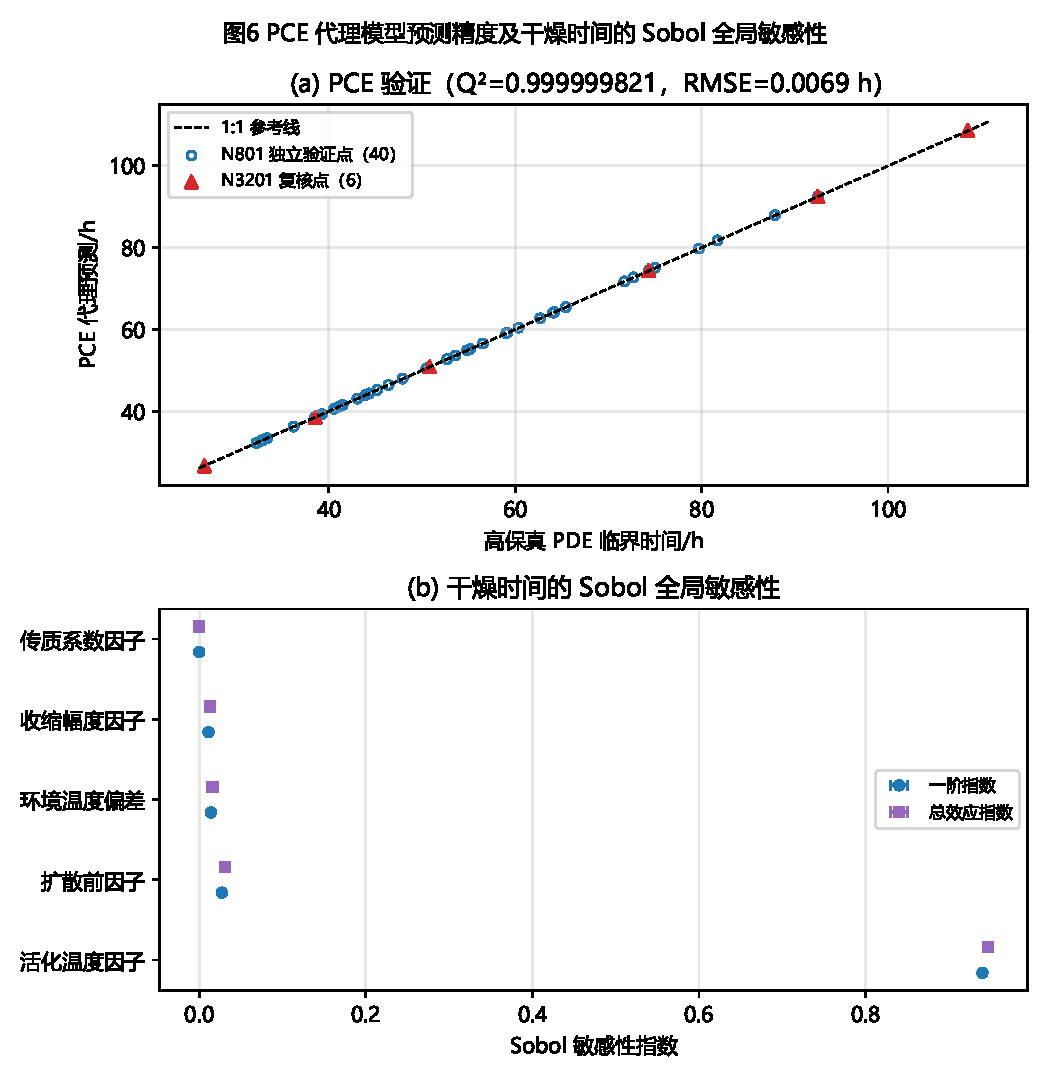
\includegraphics[width=0.88\textwidth]{../../results/paper_figures/fig5_pce_sobol.pdf}
  \caption{问题四代理模型验证与全局敏感性。(a) 4 阶多项式混沌代理预测与高保真 PDE 临界时间的对比，圆点为 40 个独立验证样本，三角为 6 个 $N=3201$ 复核样本；(b) 筛选后 5 个参数对干燥时间的 Sobol 一阶与总效应指数，误差棒为残差 bootstrap 的代理系数 $95\%$ 区间，不具有统计置信区间含义。}
  \label{fig:uq-pce-sobol}
\end{figure}

\clearpage
\section*{AI 工具使用声明}
\addcontentsline{toc}{section}{AI 工具使用声明}
本参赛队在建模与论文整理过程中使用了 AI 工具辅助代码调试、文字组织、格式检查和表达润色。AI 工具未被用于替代题意理解、模型选择、参数确认或结果判定。本文中的模型公式、参数取值、程序输出、图表数据和结论均由参赛队依据题目附件、计算程序和人工复核结果确认；若 AI 输出与题目条件或程序结果不一致，以题目附件和人工复核结果为准。

\clearpage
\begin{thebibliography}{99}
\addcontentsline{toc}{section}{参考文献}
\bibitem{cumcm2026a} 2026年全国大学生数学建模竞赛A题题目、附件及附录材料.
\bibitem{morris1991} Morris D E. Factorial sampling plans for preliminary computational experiments. \textit{Technometrics}, 1991, 33(2): 161--174.
\bibitem{xiu2002} Xiu D, Karniadakis G E. The Wiener-Askey polynomial chaos for stochastic differential equations. \textit{SIAM Journal on Scientific Computing}, 2002, 24(2): 619--644.
\bibitem{sobol2001} Sobol I M. Global sensitivity indices for nonlinear mathematical models and their Monte Carlo estimates. \textit{Mathematics and Computers in Simulation}, 2001, 55(1--3): 271--280.
\bibitem{saltelli2010} Saltelli A, Annoni P, Azzini I, Campolongo F, Riva M, Tarantola S. Variance based sensitivity analysis of model output: Design and estimator for the total sensitivity index. \textit{Computer Physics Communications}, 2010, 181(2): 259--270.
\end{thebibliography}

\end{document}



